\RequirePackage{lineno}
\documentclass[aps,prl,reprint,twocolumn,groupedaddress,showpacs]{revtex4}
\usepackage[pdftex]{graphicx}
\usepackage{epstopdf}
\usepackage{bm}
\usepackage{amssymb}
\usepackage{psfrag}
\usepackage{color}
\usepackage{amsbsy}      
\usepackage{amsmath,amsthm}
\usepackage{mathtools}
\usepackage{lineno}
\graphicspath{{./figures/}}

\newtheorem{thm}{Theorem}%
\newtheorem{lem}[thm]{Lemma}%
\newtheorem{prop}[thm]{Proposition}%
\newtheorem{coro}[thm]{Corollary}%
\DeclarePairedDelimiter{\norm}{\lVert}{\rVert}

\newcommand{\bsigma}{{\boldsymbol\sigma}}
\def\alphaeff{\alpha_{\mathrm{eff}}}
\def\a{\alpha}
\def\b{{\bf b}}
\def\c{{\bf c}}
\def\d{{\bf d}}
\def\dd{\mbox{d}}
\def\dz{\delta z}
\def\ve{\varepsilon}
\def\eps{\epsilon}
\def\f{{\bf f}}
\def\g{\gamma}
\def\r{{\bf r}}
\def\rp{{\bf r}_{\perp}}
\def\q{{\bf q}}
\def\k{\kappa}
\def\u{{\bf u}}
\def\t{{\bf t}}
\def\w{{\bf w}}
\def\x{{\bf x}}
\def\y{{\bf y}}
\def\l{\ell}
\def\o{\omega}
\def\p{{\bf p}}
\def\s{\sigma}
\def\vp{\varphi}
\def\D{\Delta}
\def\F{{\bf F}}
\def\H{{\bf H}}
\def\K{{\bf K}}
\def\L{{\bf L}}
\def\Q{{\bf Q}}
\def\S{{\bf S}}
\def\T{{\bf T}}
\def\U{{\bf U}}
\def\V{{\bf V}}
\def\W{{\bf W}}  
\def\F{{\bf F}}                
\def\P{{\bf P}}
\def\Pt{\tilde{P}}
%\def\s{\mathbf{\sigma}}
\newcommand{\bs}{\boldsymbol{\sigma}}
\newcommand{\Conv}{\mathop{\scalebox{1.5}{\raisebox{-0.2ex}{$\ast$}}}}%

%\usepackage{fullpage}
\newcommand{\RR}{\mathbb{R}}


\begin{document}

\title{High-resolution spatial reconstruction of cellular
  force-generating domains using physical constraints and rotationally invariant $L^{1}$
  regularization}

\author{Joshua C. Chang$^{1}$, Yanli Liu$^{2}$, and Tom Chou$^{2,3}$}
\affiliation{$^{1}$Epidemiology and Biostatistics Section, Rehabilitation
  Medicine, Clinical Center, The National Institutes of Health,
  Bethesda MD, 20892} \affiliation{Dept. of Mathematics, UCLA, Los Angeles, CA 90095-1555}
\affiliation{Dept. of Biomathematics, UCLA, Los Angeles, CA 90095-1766}

%\maketitle 

%\begin{article}


%\runninglinenumbers*

\begin{abstract}
We develop a method to reconstruct, from measured displacements of an
underlying elastic substrate, the spatially dependent forces that
cells or tissues impart on it.  Given newly available high-resolution
methods to image substrate displacements, it is desirable to be able
to reconstruct small scale, compactly supported focal adhesions, which
are localized and can exist only within the footprint of the cell or
tissue.  We solve this inverse problem using methods of convex
regularization. In addition to the standard quadratic data mismatch
terms that defines least-squares fitting, we motivate a term in the
objective function which penalizes variations in the vectorial invariants
of the reconstructed surface stress while preserving boundaries.  By
minimizing the objective function subject to appropriate physical
constraints, we are able to efficiently reconstruct stress fields with
localized structure from simulated and experimental substrate
displacements. We provide a numerical method for setting up a
discretized inverse problem that is solvable by standard convex
optimization techniques. Our method incorporates the exact solution
for the stress tensor accurate to first-order finite-differences,
motivates the use of distance-based cutoffs for data inclusion, and
finds--under loose regularity conditions--the reconstruction error
that results.
\end{abstract}
\maketitle

\section{Introduction}

The adhesion of cells and tissues to their environment has profound
consequences on processes such as cell polarization \cite{MASHA2011},
division, differentiation \cite{DIFFERENTIATION0}, tissue morphology
during development \cite{DEVELOPMENT0}, wound healing
\cite{WOUND0,WOUND2,WOUND1}, and cancer metastasis
\cite{CANCER0}. Hence, quantifying how cells attach to an impart force
on the surrounding material is an important technical challenge in
cell biology.

Cell motility and response to signals have hitherto typically been
studied in two-dimensional geometries in which cells are placed on a
flat elastic substrate.  Dynamic adhesion between the cells and the
substrate are realized through {\it e.g.}, lamellapodia, filapodia,
and dynamically reorganizing focal adhesions \cite{MBOC}.  Such structures are
spatially localized, as shown in Fig.~\ref{FIG1}. Similarly, on larger
length scales, a collection of cells can give rise to localized stress
distributions. For example, the leading edge of a cell layer produces
the pulling force that leads to migration in wound healing assays.

\begin{figure}[t]
\begin{center}
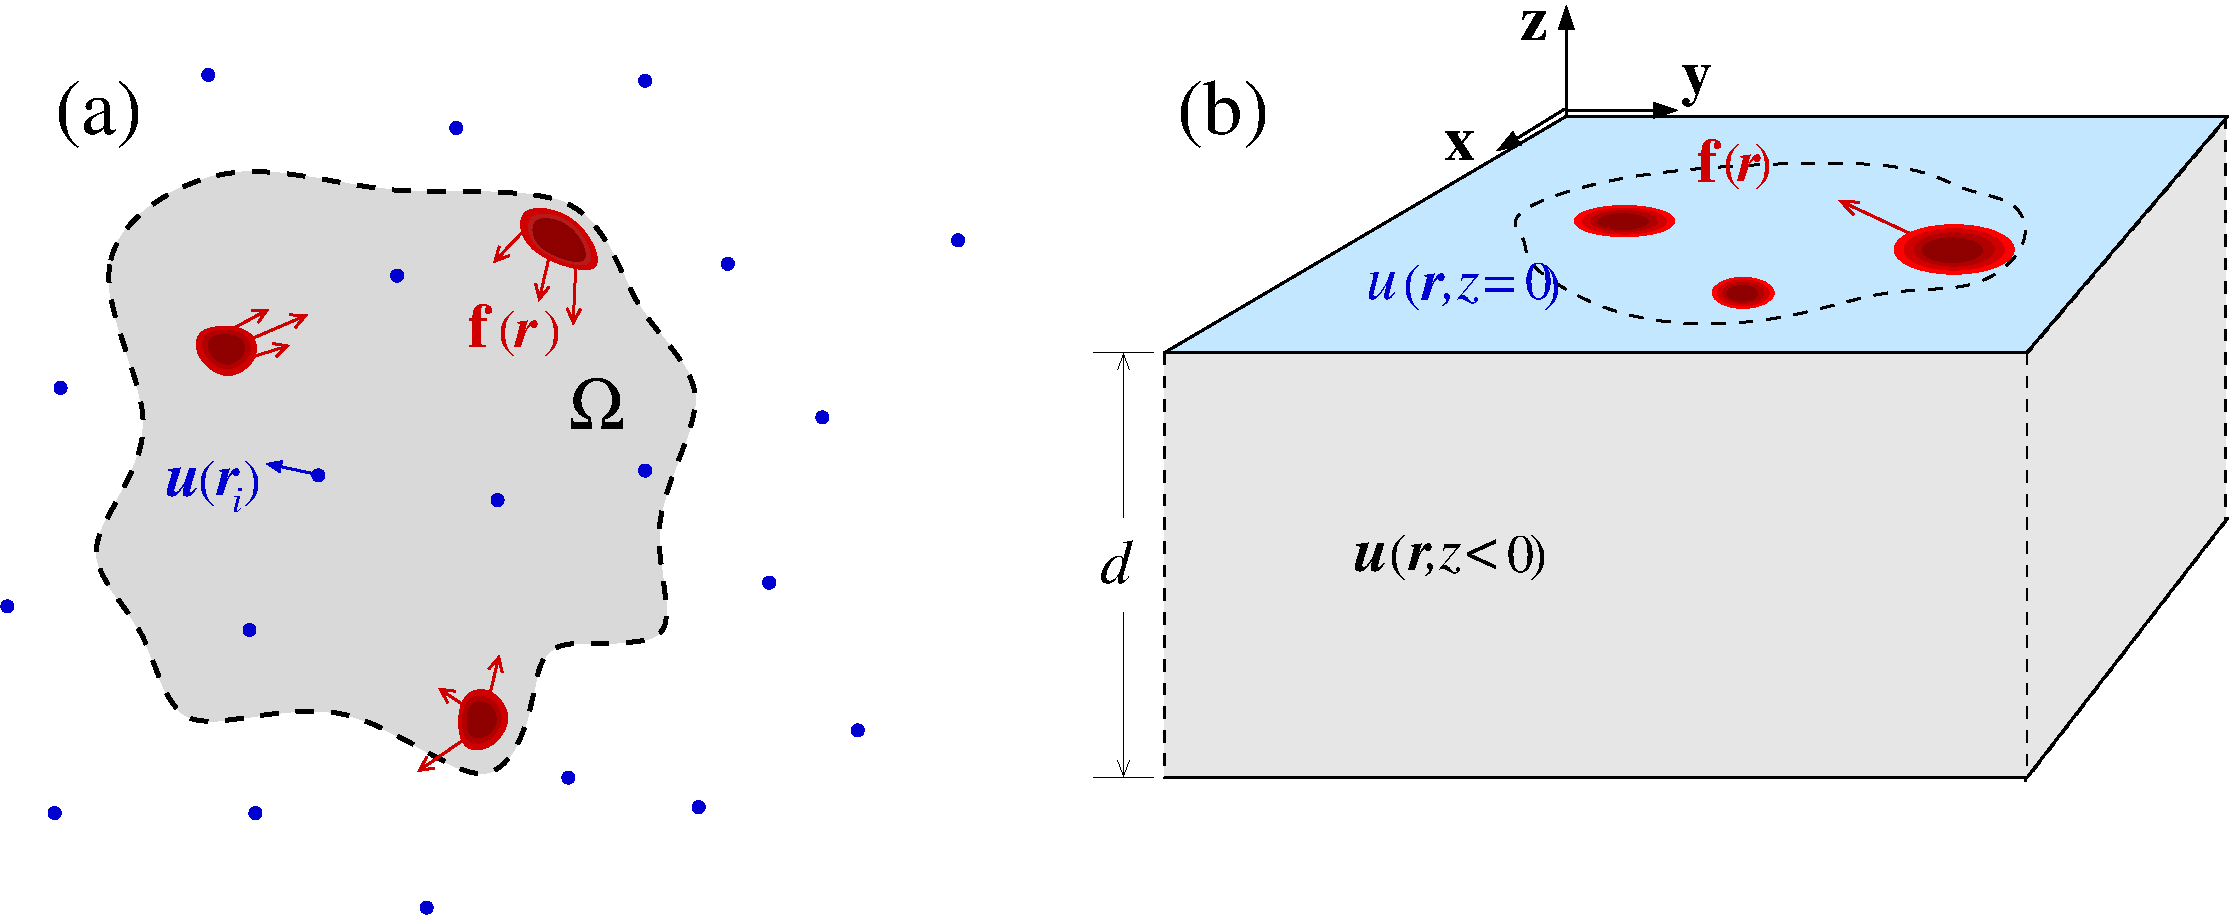
\includegraphics[width=\linewidth]{Fig1.pdf}
\caption{A schematic of an isolated cell. (a) The boundary of the cell
  footprint is denoted by the dashed curve, the support of the stress
  field is represented by the red regions that impart a stress ${\bf
    f}(x,y)$ on the surface. Displacements ${\bf u}(\r_{i})$ of the
  elastic medium are measured at position $\r_{i} =
  x_{i}\hat{x}+y_{i}\hat{y}+z_{i}\hat{z}$ (blue dots) that can be
  inside or outside the cell footprint, on the surface ($z_{i}=0$), or
  below the surface ($z_{i}<0$). (b). A perspective view of the
  elastic substrate and cellular footprint.}
\label{FIG1}
\end{center}
\end{figure}

Dynamically varying force-generating structures are often small and
difficult to image, especially without biochemical modification such
as incorporation of fluorescent dyes. Therefore, other methods for
inferring their positions and magnitudes have been developed. Methods
using deformation of pillar structures \cite{PILLAR} or textured
substrates have been developed \cite{PATTERN}.  These methods require
the cell to attach to a nonflat interface.  The simplest method
compabible with a flat interface relies on measuring the displacement
of fiduciary markers, such as gold nanoparticles, embedded in the
elastic substrate~\cite{WANG2007}. The measured displacements are an
indirect probe of the force-generating structures, \textit{e.g.},
focal adhesions.  Any inversion method should be able to not only
reconstruct the positions and magnitudes of the stress field, but
should ideally be able to capture potentially sharp boundaries of the
stress-generating structures. However, fiduciary markers embedded in
the 3D substrate are typically too sparse to reveal a displacement
field with sufficient resolution to infer small cellular focal
adhesion structures. To image such subcellular stress structures, high
resolution reconstructions are required \cite{USCHWARZ}.
Experimentally, a new high-resolution imaging method has been
developed using 9$\mu$m-period grid patterning of the substrate
\cite{POPESCU}.  A surface grid pattern of fluorescent adhesion
proteins allows surface deformation to be directly measured using
conventional microscopes.

In light of such higher spatial resolution techniques, we develop a
novel method for elastic stress source recovery using ideas developed
for image segmentation \cite{OSHER}.  This class of methods relies on
optimization that uses an $L^{1}$ regularization term in the objective
function \cite{CHAN}.  This type of regularization term is not derived
from any fundamental physical law, but represents a prior knowledge that
the function to be recovered is sparse in content except near
edges. In addition, the overall objective function will be constructed
to obey physical constraints and symmetries.

In the next section, we review the standard linear equations of
elasticity that describe the displacement field as a function of an
arbitrary surface stress distribution. This model is then used to
construct the data mismatch term in the objective function. We then
motivate regularization and constraint terms in the full
objective function. Finally, we demonstrate our method
using both simulated and experimental data. Our method provides
good reconstruction of localized structures that exhibit desirable
qualities such as the suppression of Gibbs ringing phenomenon at the
boundaries of the stress structures.


\section{Elastic Model}

We first derive the linear elastic Green's function associated with a
point force applied to the surface of a semi-infinite half-space, as
shown in Fig.~\ref{FIG1}(b). We assume that the elastic medium is
infinite in both depth ($d\to \infty$) and lateral extent. The Green's
function tensor defined in the domain ${\cal D}=\left\{(x,y,z)|x,y\in
R,z\leq0\right\}$ is given by
\begin{equation}
{\bf G} = \left[ \begin{matrix} G_{xx}(x,y,z) & G_{xy}(x,y,z) & G_{xz}(x,y,z) \\
	G_{yx}(x,y,z) & G_{xy}(x,y,z) & G_{yz}(x,y,z) \\
	G_{zx}(x,y,z) & G_{zy}(x,y,z) & G_{zz}(x,y,z) 
 \end{matrix} \right]
\end{equation}
where the components are explicitly given in 
Appendix A. For example, 

\begin{equation}
G_{sz, zs}(x,y,z) =
\frac{1+\nu}{2\pi E}\left(\frac{sz}{R_{\perp}^{3}}\pm\frac{(1-2\nu)s}{R_{\perp}
(R_{\perp}-z)}\right).
\end{equation}
%
where $s\equiv x,y$. The equation with $\pm$ corresponds to $G_{sz}$
and $G_{zs}$, respectively, and $R_{\perp} \equiv \sqrt{x^{2}
  +y^{2}}$. The Young's modulus and Poisson ratio of the elastic
substrate are denoted by $E$ and $\nu$, respectively.  For Matrigel,
$E\approx4\pm3\times10^2\textrm{ Pa}$ and
$\nu\approx0.5$~\cite{SOOFIA2009}. Throughout the rest of this
manuscript, we will express stress in units of $E$.  The displacement
of a material point at $(x,y,z\leq 0)$ in the medium due to a stress
distribution ${\bf f}$ is simply the convolution $\u(\r) \equiv [u_x
  \ u_y\ u_z]^\intercal = {\bf G}\Conv\f$.
%
%, while for a surface-localized force distribution, 
%$\F=(F_{x}(x,y,z=0),F_{y}(x,y,z=0),F_{z}(x,y,z=0))$ the displacement would be

%\begin{equation}
%\left[\begin{array}{c} u_{x}\\u_{y}\\u_{z}\end{array}\right]=
%\left[\begin{array}{ccc} G_{xx}&G_{xy}&G_{xz}\\G_{yx}&G_{yy}&G_{yz}\\G_{zx}&G_{zy}&G_{zz}
%\end{array}\right]
%\left[\begin{array}{c} F_{x}\\F_{y}\\F_{z}\end{array}\right]
%\end{equation}
%
%
%For a force distributation
%
%\begin{equation}
%\F=(F_{x}(x,y),F_{y}(x,y),F_{z}(x,y)) 
%\end{equation}
% 
%exerting on the surface of the medium,the displacement would be:
%\begin{equation}
%u_{i}(\r) = \int \dd \r_{\perp}'\dd z'
%G_{ij}(\r_{\perp}-\r_{\perp}',z-z')
%F_{j}(\r_{\perp}', z'),
%\label{UMODEL0}
%\end{equation}
% 
%where $\r = (\r_{\perp},z)$, $\r_{\perp}=x\hat{x} + y\hat{y}$ and
%$\r_{\perp}'= x'\hat{x} + y'\hat{y}$.  We will use this expression for
%the displacement as the model for the data term in the objective
%function for our inverse problem.


For our specific problem, we shall restrict the forces to surface
stresses $\f$ that act on the plane perpendicular to the
$\hat{z}$ axis. We define the in-plane stress distribution, at depth $z$, as
$\f(x,y) = f_{x}(x,y)\hat{x} + f_{y}(x,y)\hat{y}$. 
The resulting surface-level displacement fields become

\begin{equation}
u_{s}(x,y,z) = \sum_{k=x,y,z}\int_\Omega \dd x'\dd y'G_{sk}(x-x',y-y',z)f_{k}(x',y').
\label{eq:UMODEL1s}
%\nonumber\\
%&\qquad +  \int_\Omega \dd x'\dd y'G_{xy}(x-x',y-y')\sigma_{yz}(x',y') \label{eq:UMODEL1x}  \\
%u_y(x,y) &= \int_\Omega \dd x'\dd y'G_{yx}(x-x',y-y')\sigma_{xz}(x',y') \nonumber\\
%&\qquad +  \int_\Omega \dd x'\dd y'G_{yy}(x-x',y-y')\sigma_{yz}(x',y'),  \label{eq:UMODEL1y}  
\end{equation}
%
%where $G_{ij}(x,y) \equiv G_{ij}(x,y,z=0)$ and $\sigma_{sz}(x,y)
%\equiv \sigma_{sz}(x,y,z=0)$.  
Note that tangential stresses can induce
displacements in the direction normal to the surface.
For cells on flat surface, we assume that $f_{z}=0$.
\section{Inverse problem}

Next, we develop an objective function for which the minimizing
solution provides a good approximation to the underlying stress field,
while preserving discontinuities.  The first component is simply a
quadratic data mismatch term defined by the sum over the displacements
measured at the $N$ measurement positions at $\r_{i}$:

\begin{equation}
\Phi_{\rm data}[\f] = \sum_{i}^{N}\vert \u^{\rm
  data}(\r_{i})- \u(\r_i\vert \f)\vert^{2}.
\label{PHIDATA}
\end{equation}
%
Since $\u^{\rm data}(\r_{i})$ is given, and $\u(\r_{i}\vert \f)$ is
given by the linear model of Eq.~\ref{eq:UMODEL1s}, this contribution
to the objective function is a functional over the surface force
$\f(x,y)$.  For simplicity, we will assume that the data points are
measured only at the interface $z=0$ over an uniform grid with
coordinates given $\{ (x_j,y_k) : j\in\{1,2,\ldots,J\},
k\in\{1,2,\ldots,K\}\}.$

In Eq.~\ref{eq:UMODEL1s}, we have restricted the domain of integration
to lie within the cell footprint $\Omega$, further emphasizing that
$\f(x,y)$ has compact support. As a consequence of compact
support, for a fixed, discretized approximation of
$\f(x,y)$, the displacements can be obtained exactly
by solving an equivalent system of linear equations of finite
dimension.

Here, we explicitly define this system of linear equations given a
piecewise-affine approximation of the stress field. Let us consider
the first-order approximation of $f_{x}(x,y)$ and $f_{y}(x,y)$ using
central finite differences, for $x\in[x_j - \delta x/2, x_j+\delta
  x/2) \cap y\in[y_j-\delta y/2, y_j + \delta y /2)$,
\begin{align}
\lefteqn{f_{x}(x,y) =f_{x}(x_i , y_j)  }\nonumber \\
& \qquad+ (x-x_i)\frac{f_{x}(x_{i+1},y_j) -f_{x}(x_{i-1},y_j) }{2\delta x}  \nonumber\\
&\qquad + (y-y_j)\frac{f_{x}(x_i,y_{j+1}) - f_{x}(x_i,y_{j-1}) }{2\delta y} \nonumber\\
&\qquad + \mathcal{O}(\delta x)^2 + \mathcal{O}(\delta y)^2,\label{eq:sigma_affine}
\end{align}
where $i,j$ denotes a tuple of grid coordinates. In effect, we are
performing sub-pixel interpolation of the stress where the stress is
fully-determined by its values at the grid vertices.

Upon using Eq.~\ref{eq:sigma_affine}, we can rewrite
Eq.~\ref{eq:UMODEL1s} by decomposing the integral into a sum of
integrals over grid cells.  After further regrouping terms, we find a
linear system of equations for $u_{s}(x,y)$ at all grid points
simultaneously. For example, 

\begin{equation}
u_{x}(x_{n},y_{m}) = X^{nmjk}f_{x}(x_j,y_k) + Y^{nmjk}f_{y}(x_j,y_k),
\label{eq:linearsystem1}
\end{equation}
%
where the tensors $X^{nmjk}$ and $Y^{nmjk}$ are given in Appendix B and 
summation notation for each index tuple $(j,k)$ has been implicitly assumed.

From an equation-counting perspective, the system of equations is
exactly determined given that one has at least as many measurement
points as grid cells in the resolution that one wishes to reconstruct
the stress field, provided that one is able to measure displacements
in both principle directions. Even if one is able to measure both
displacements, the problem may still be difficult since the inversion
of Eq.~\ref{eq:linearsystem1} maybe highly ill-conditioned and the
measurements are taken in the presence of noise at a finite
precision. To resolve these issues, we introduce a number of
physically consistent constraints and regularization terms relevant to
this system.

\subsection{Physical constraints and regularization}

The remaining components of the objective function should contain
information about the the known physical constraints as well as
regularization terms that better condition the overall optimization
problem. Various regularization terms have been motivated, but they
can also be associated with prior knowledge on the solution
\cite{PATHINTEGRAL}. 

First, we consider explicit physical constraints. Since we are
assuming inertial effects are negligible, we require that the net
force is zero, or that
\begin{equation}
\int_\Omega f_{x}(x,y)\dd x \dd y= \int_\Omega f_{y}(x,y)\dd x \dd y = 0.
\label{NOFORCE}
\end{equation}
Likewise, we require that there is no net torque, or that
\begin{equation}
\int_\Omega x f_{y}(x,y) \dd x \dd y  = \int_\Omega y f_{x}(x,y) \dd x \dd y.
\label{NOTORQUE}
\end{equation}
%
Another physical constraint is the requirement that surface stress at
locations outside of the cell footprint vanish.  In regions where
there is no contact between the cell and the substrate, no mechanism
can impart stress.  Thus, the stress field is compactly supported
within the cell footprint.  The stress field may be further localized
through cellular focal adhesions within the cell footprint

To better condition the inference of $\f(x,y)$, we regularize
this problem by forcing the reconstruction to obey some physically
relevant characteristics of the surface stress. In many other types of
inverse problems, for example, in the inference of the potential of
mean force of a molecular bond, a contraint on differentiability is
typically imposed on the function to be inferred \cite{PATHDFS}. A
typical constraint of this nature may be a quadratic penalty on the
gradients of the function to be inferred.  However, such $L^{2}$
functional regularization often leads to ringing and inaccurate
functional reconstruction especially when the underlying function is
highly localized or compactly supported.

Thus, $L^{1}$ regularization on the function or on its variations have
been developed.  These approaches are suitable for problems such as
segmentation of images where boundaries are are sharp \cite{CHAN}.  In
these problems, the data is sparse in the sense that definition of
boundaries in an image contain most of the information.  Likewise, in
the stress recovery problem at hand, the data consisting of
displacements at a finite number of measurement positions may be
considered sparse.

%We also compared reconstruction of the surface stress using our
%rotationally invariant norms of Eq.~\ref{eq:PhiL1Tr} and
%Eq.~\ref{eq:PhiTVTr} against alternate isotropic norms. As an
%alternative to the $L^1$ norm on the trace we compared

To this end we employ a variant of a penalty used often in
image processing applications, where one penalizes the $L^1$
norm of the variation in the fields, or the total variation.
In analogy with image processing, one might choose regularization terms 
$\Phi_{\rm reg}$ of the form

\begin{equation}
\Phi_{L^{1}} = \int_\Omega \left(\vert f_{x}(x,y)\vert  +\vert f_{y}(x,y)\vert\right) \d\r,
\label{L10}
\end{equation} 

\begin{equation}
 \Phi_{{\rm TV}_1} = \int_\Omega \left( \vert\nabla f_{x}(x,y) \vert +
 \vert\nabla f_{y}(x,y) \vert\right)\d\r
 \label{eq:PhiTV1}
\end{equation}
and
\begin{equation}
\Phi_{{\rm TV}_2} = \int_\Omega \left(\vert\partial_x f_{x}\vert 
+ \vert\partial_y f_{x}\vert + \vert\partial_x f_{y}\vert
+ \vert\partial_y f_{y}\vert\right)\d\r,
 \label{eq:PhiTV2}
\end{equation}
%
representing an $L^{1}$ regularization of the surface stress and two
forms of its total variation, respectively.  Since these
regularization terms are not based on any fundamental physical law,
there is some freedom of in choosing their form.  However, we do not
want rotational anisotropy in the measurement grid to affect the final
result. The regularization terms should not induce any additional
anisotropy over that of the displacement field.  Thus, appropriate
regularizations should be invariant under coordinate rotation. The
coordinate-independent regularizer can be 
constructed from the magnitude of the force vector at the surface
\begin{equation}
\vert\f(x,y) \vert  = \sqrt{f_{x}^{2} + f_{y}^{2}}.
\end{equation}

%Similarly, for the variation of $\bsigma$, the trace and determinant
%of $\partial_{i}\sigma_{jz}$ are rotational invariants:

%\begin{equation}
%\textrm{Tr}(\nabla \bsigma) = \partial_{x}\sigma_{xz} + \partial_{y}\sigma_{yz},
%\end{equation}

%\begin{equation}
%\textrm{Det}(\nabla\bsigma) = \partial_{x}\sigma_{xz} \partial_{y}\sigma_{yz}-
%\partial_{x}\sigma_{yz}\partial_{y}\sigma_{yz}.
%\end{equation}
%
Any regularization penalty imposed on the reconstruction problem must
be a functional of these invariants in order to maintain rotational
invariance relative to the choice of how the displacements are
sampled.  In this manuscript, for simplicity, we will focus on
regularizers $\Phi_{\rm reg} = \tilde{\Phi}_{\rm reg}$ that are functions of the magnitude and
trace; for example
\begin{equation}
\tilde{\Phi}_{L^{1}} = \int_\Omega \vert\f(x,y) \vert \dd x\dd y
\label{eq:mag}
\end{equation}
and
%
\begin{equation}
\tilde{\Phi}_{\rm L^2} =  
 \int_\Omega \vert\f(x,y) \vert^2 \dd x\dd y.
\label{eq:PhiTVTr}
\end{equation}

Using either of these expressions as the regularization norm
suggests the penalized optimization problem

\begin{equation}
\hat{\f} \big\vert \lambda = \arg\min_{\f} \left\{ \Phi_{\textrm{data}}[\f] + 
\lambda\Phi_{\textrm{reg}}[\f] \right\},
\label{eq:objective}
\end{equation}
%
subject to the no-force, no-torque, and footprint constraints
(Eqs.~\ref{NOFORCE} and \ref{NOTORQUE}) on $\f$ mentioned above.
In Eq.~\ref{eq:objective}, $\lambda>0$ is a tunable parameter. This
problem is in a standard form that is directly solvable using a
variety of optimization routines.  In our implementation, we use a
second-order quadratic cone solver~\cite{cvxpy}.

%\subsection{Numerical cut-off and error}
To reduce the size of the system of equations described in
Eqs.~\ref{eq:linearsystem1}, we note that the Green's function falls
off at a rate of $|\r|^{-1}$. However, when combined with the
zero-force constraint, the relationship between the
displacements and the support of the stress field falls off at the
much quicker rate of $|\r|^{-2}$. Formally, if 
%
% under a set of reasonable
%assumptions that are consistent with the choice of regularization that
%we have made.
%
$\Omega = {\rm sup}(\bsigma)\subset \mathbb{R}^2$ is compact, and
 $\int \bsigma(\r)\d\r = \mathbf{0}$, then
as $\mathbf{r}\to\infty$, $u_{x,y}(\r) = \mathcal{O}\left( |\r|^{-2} \right)$.

% For a fixed
%$\mathbf{x}\not\in\Omega$, denote $D(\mathbf{x}) = \inf\{ ||
%\mathbf{x} -\mathbf{y}|| : \mathbf{y}\in\Omega \}$. Then, for
%$\mathbf{x}$ where $D(\mathbf{x})\geq R>0$,
%\begin{equation}
%\vert u_x(\mathbf{x}) \vert \leq \frac{C_x\norm{\bsigma}_1}{R^2}
%\end{equation}      
%and
%\begin{equation}
%\vert u_y(\mathbf{x}) \vert \leq \frac{C_x\norm{\bsigma}_1}{R^2}
%\end{equation}      
%for some constants $C_x,C_y$.

%Furthermore, if $\tilde{\bsigma}$ is an affine approximation to
%$\bsigma\in C^s(\Omega)$ for $s\in\mathbb{Z}^+$, and $\tilde{\u}$ is
%the corresponding displacement field generated from $\tilde{\bsigma}$,
%
%\begin{equation}
%\vert \tilde{\u}  - \u \vert \leq C (\delta x)^2
%\end{equation}

The decay of the influence of stress on the system provides
justification for setting distance-based cut-offs of the linear
system. The effect of the cut-off is to limit the left-hand side of
Eq.~\ref{eq:linearsystem1} to locations only within some maximal
distance $R_{\perp}$ from the outline of the cell.

%The error in the solution of the inverse problem is dependent on the
%precision of the observations, the physical constants that describe
%the medium, and the maximum magnitude of the stress. The error from
%cutting off the domain over which displacements are used in the
%reconstruction of $\bsigma(\r)$ can also be bounded. If
%Define $\hat{\bsigma}^R(\r)$ as the reconstructed stress field found by
%solving the optimization problem of Eq.~\ref{eq:objective} using only
%the displacement data within a maximal distance of $R$ from the
%cell. In Appendix C, we show that 
%%Denote $\varepsilon^R(\r) = \hat{\bsigma}^R(\r) - \bsigma(\r)$ for
%%$\r\in\Omega$, where $\sigma_{xz}\in L^1(\Omega)$,
%\begin{equation}
%\sup \vert \hat{\bsigma}^R(\r) - \hat{\bsigma}^\infty(\r) \vert \leq \frac{C}{R^2}
%\end{equation}



\section{Results}

We implemented our regularized inversion method in Python version 3.5,
where optimization is performed using the \texttt{cvxpy} package with
the \texttt{ecos} solver.  Our implementation is available at
\url{https://github.com/joshchang/tractionforce}. 

\begin{figure*}[ht]
\begin{center}
\includegraphics[width=5.2in]{fig2.pdf}
%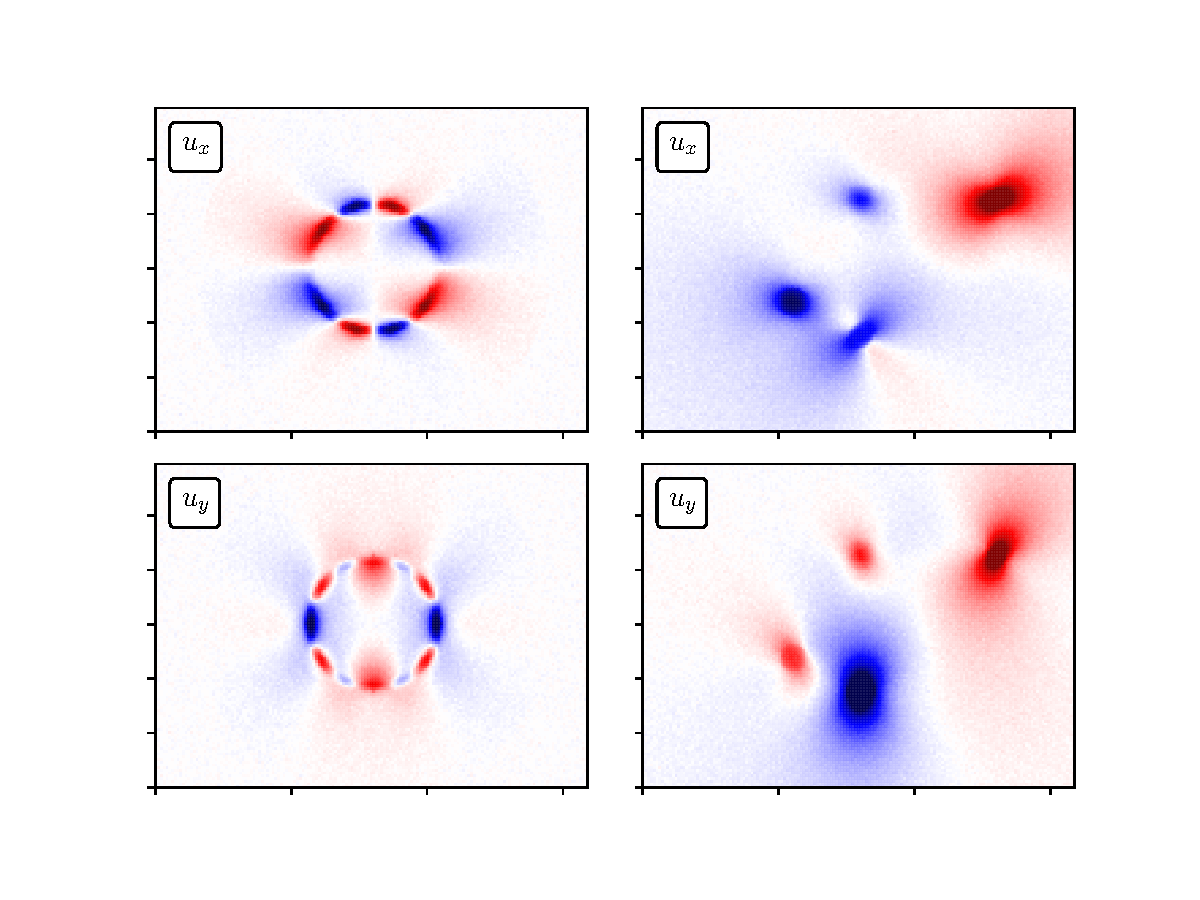
\includegraphics[width=4.2in]{displacements}
%
\caption{\textbf{Test stress fields and surface displacements.} (a)
  Four focal adhesions attached by filaments indicated by the green
  lines. The red border represents the extent of the cell footprint
  and can be determined experimentally as part of the imaging.
  Mathematically, the cell boundary forms the basis for a constraint
  on the stress distribution and we explore the dependence of the
  quality of reconstruction on the footprint constraint. The faint
  blue grid represents the regular points at which displacements might
  be measured. (b) and (c) show the corresponding surface
  displacements $u_{x}(x,y)$ and $u_{y}(x,y)$,
  respectively.\label{TEST}}
\end{center}
\end{figure*}
%\end{widetext}
%

First, we tested our method on simulated data derived from a force-
and torque-free test stress field shown in Fig.~\ref{TESTS}. The test
pattern consists of four separated circular stress pads, or focal
adhesions, with radii $r_{1} = 1/5$, $r_{2} = 1/6$, $r_{3} = 1/8$, and
$r_{4} = 1/4$, and centers at positions $(x_{1},y_{1}) = (-1,-1/2)$,
$(x_{2},y_{2}) = (0,-1)$, $(x_{3},y_{3}) = (2,1)$, and $(x_{4},y_{4})
= (0,1)$.  The pads 2,3, and 4 are connected in a triangle as shown,
while pad 1 is connected only to pad 2.  The tensions along these
connections give rise to surface stresses imparted by the pads onto
the substrate.  We will assume that the stress fields in pads 1,2, and
3 are uniformly distributed within the circular disks. For pad 4, we
assume that the filaments connected to it distributed according to a
cone-like density function. Thus, the stress field within pad 4
linearly decrease along the radial direction. The stresses $\f^{(i)}$
under each patch $i$ are decomposed into contributions arising from
the total tension $T_{ij}$ connecting them with pad $j$ and can be
expressed in the form

\begin{align}
\f^{(1)} & = a_{12}\left(\hat{x} -{\hat{y}\over 2}\right) \label{SIGMA1}\\
\f^{(2)} & = {G_{4}\over A_{2}}\hat{y} - a_{12}{A_{1}\over A_{2}}\left(\hat{x} 
-{\hat{y}\over 2}\right) + a_{23}(\hat{x}+\hat{y}) \label{SIGMA2} \\
\f^{(3)} & = -\hat{x}{G_{4}\over A_{3}} - a_{23}{A_{2}\over A_{3}}(\hat{x}+\hat{y}) 
\label{SIGMA3}\\
\f^{(4)} & = g_{4}\left(1- {r \over r_{4}}\right)(\hat{x}-\hat{y})\label{SIGMA4}
\end{align}
%
where $a_{12}, a_{23}, g_{4} >0$ are constant amplitudes, 
$A_{i} = \pi r_{i}^{2}$ are the pad areas, and 

\begin{equation}
G_{4} = 2\pi g_{4}\int_{0}^{r_{4}}\left(1-{r\over r_{4}}\right)r\dd r = {g_{4}\pi r_{4}^{2}\over 3}
\end{equation}
%
is the total force on pad 4 in each direction. Note that both test
stress fields are constructed to be force- and torque-free. We first
generate the displacement fields using the Green's function 
(\textit{i.e.}, Eq.~\ref{eq:UMODEL1s} for surface values $\u(x,y,z=0)$)
and then recover $\f(\r)$ from these displacements.

%\begin{figure}[t]
%\begin{center}
%\input{Fig1.pstex_t}
%\includegraphics[width=3.4in]{}
%\caption{\textbf{Inversion results for test stress fields.} (a)
%  Inversion for the annular stress field with $m=3$, $n=5$ and
%  ...using different cell boundaries.... }
%\label{RESULTS_TEST}
%\end{center}
%\end{figure}

\begin{figure}
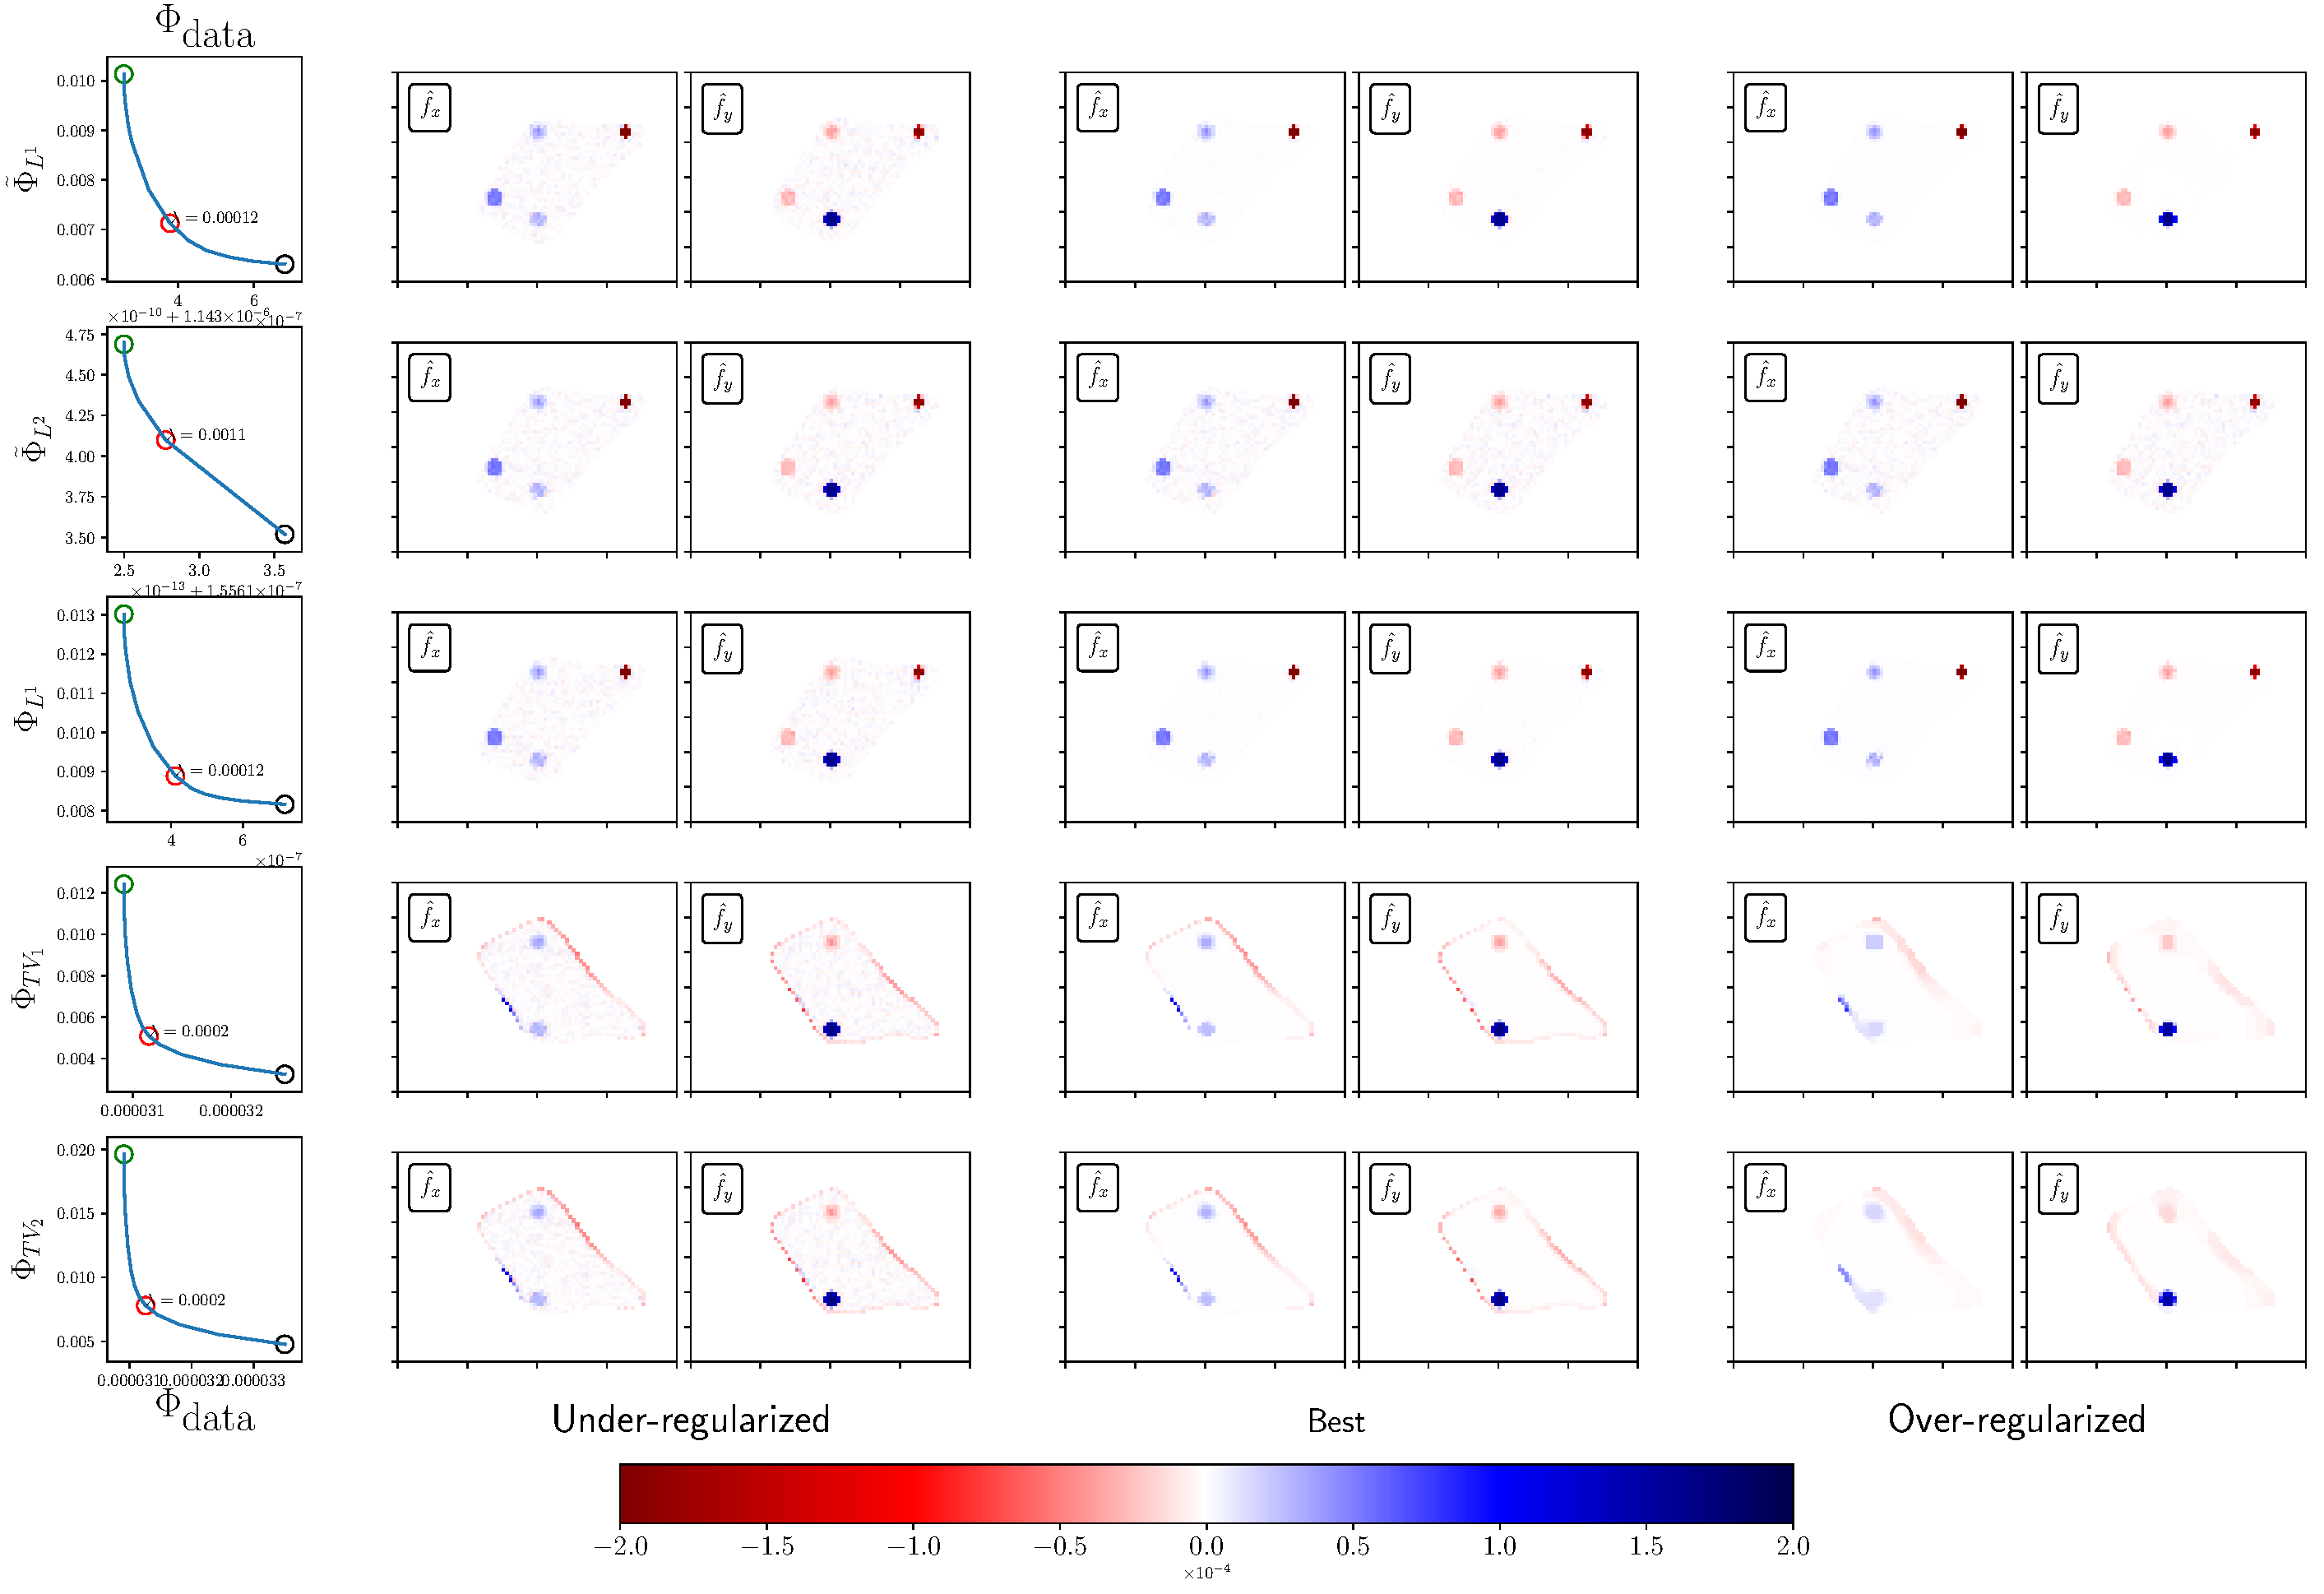
\includegraphics[width=\linewidth]{fig3}
\caption{\textbf{Comparing different regularizers.} Reconstruction of the test
  patterns using the different forms of $\Phi_{\rm reg}$:
  $\Phi_{L^{1}},\Phi_{{\rm TV}_1},\Phi_{{\rm TV}_2}$,$\tilde{\Phi}_{L^{1}}$ and
  $\tilde{\Phi}_{\rm {TV}_{1}}$. The optimal values of $\lambda$ are shown
  in.....}
\label{COMPARE}
\end{figure}
%
Figure~\ref{COMPARE} compares the reconstruction achieved from using
the different forms of $\Phi_{\rm reg}$. We see that 
all forms of regularization give reasonable reconstructions but ....
%
%that 
%$\Phi_{L^{1}}$ gives a more ``compressed'' reconstruction than 
%$\Phi_{L^{1}{\rm (Tr)}}$.  
\vspace{1cm}
%
In all of these reconstructions, we have imposed that the surface
stress is both force-free and torque-free, and also that the support
of the stress is within given cell boundaries.

The adjustable parameter $\lambda$ was chosen in each instance by
examining the balance between data mismatch and regularity using
trade-off curves shown in Fig.~\ref{COMPARE}, and taking the value
for $\lambda$ that yields a point farthest away from the line segment
joining the ends of the plot. In Fig.~\ref{compare}, the chosen value
of $\lambda$ corresponds to the given balance between regularity and
data fidelity marked by the red circle. The solution corresponding to
this particular value of $\lambda$ is shown in the middle column on
the right. For reference, under-regularized solutions, corresponding
to the green circle in the trade-off plot, and over-regularized
solutions, corresponding to black circle, are also given. Each row in
Fig.~\ref{compare} corresponds to the use of a different
regularization penalty functional. 

Figure \ref{GRID} shows reconstructions of the 4-pad test patterns
using $\tilde{\Phi}_{L^{1}}$ as a function of the coarseness of the
displacement data. The general features of the stress patterns are
preserved under coarsening but sufficient density of data points are
needed to resolve fine scale variations in the stress field. Here, we
applied the boundary constraint corresponding to the cell footprints
shown in Fig.~\ref{TEST}(a).

\begin{figure}
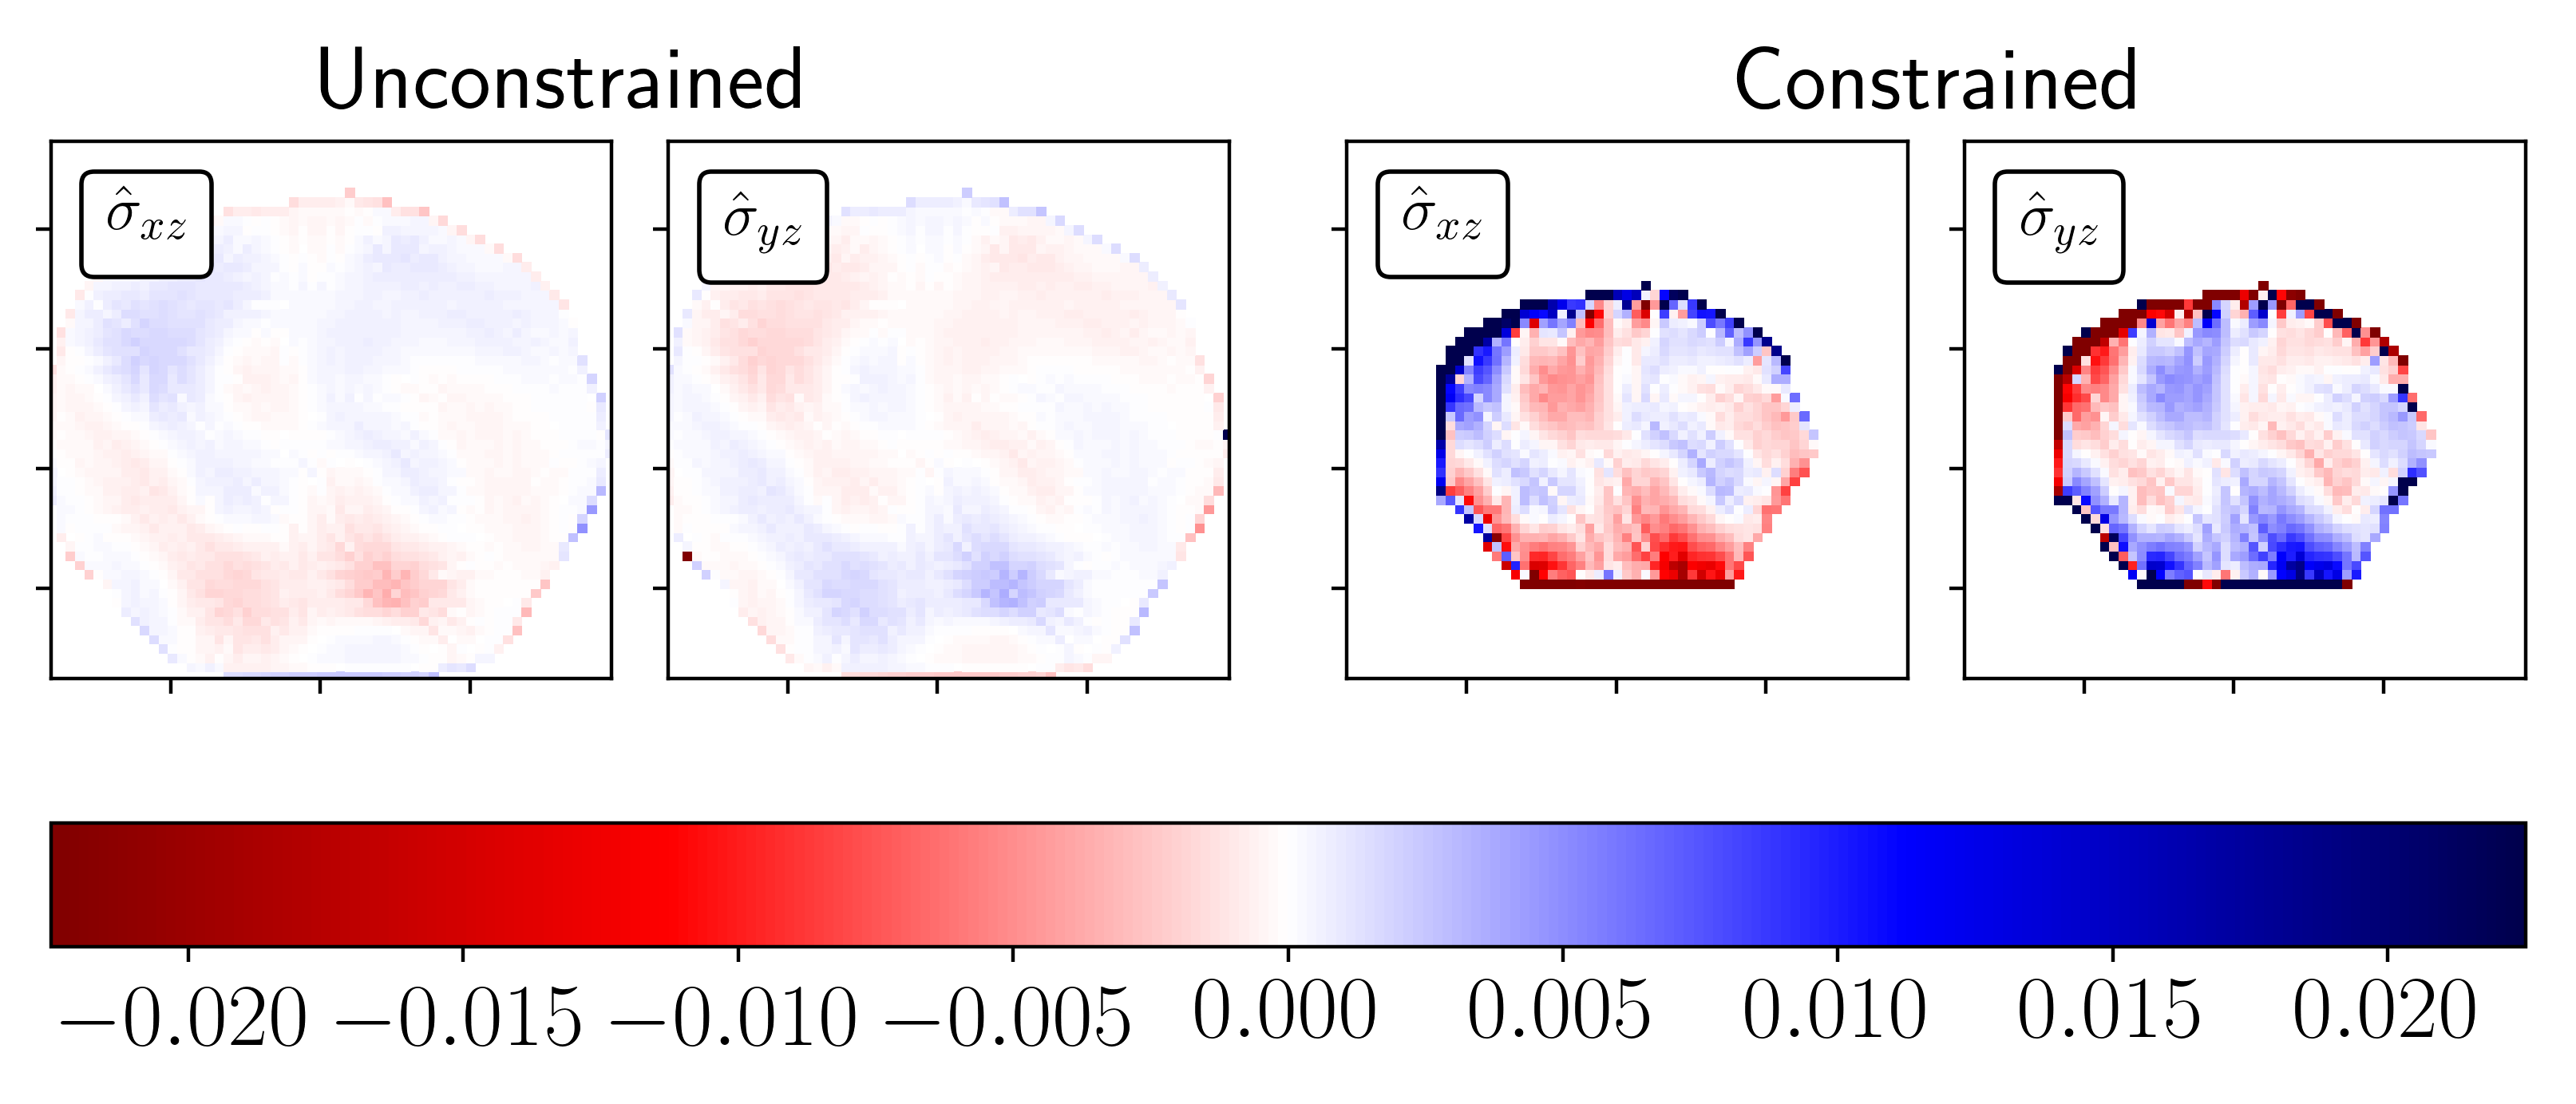
\includegraphics[width=\linewidth]{fig4}
\caption{\textbf{Grid coarsening.} Using every $n\in\{1,2,4\}$
  lattice points of observations. The reconstruction is also performed
  at the same resolution.  In general, the optimization is stable and
  the qualitative features of the reconstructed $\f(x,y)$ are robust
  to modest data coarsening.}
\label{GRID}
\end{figure}

We also test loss of information by assuming that 
displacements only in the $\hat{x}$ or $\hat{y}$ directions 
are measured. In Fig.~\ref{XYONLY} we show reconstructions using only 
$u_{x}$ or $u_{y}$ for both the annulus and 4-pad test patterns.

\begin{figure}
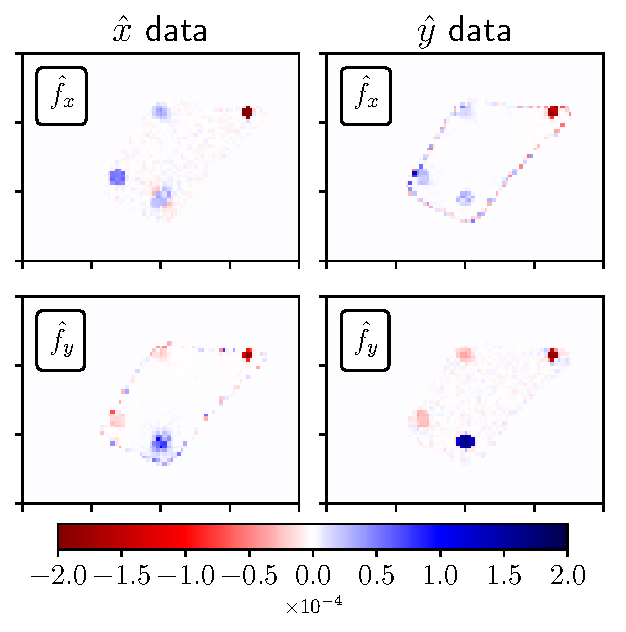
\includegraphics[width=\linewidth]{fig5}
\caption{\textbf{Unidirectional displacement measurements,} where displacements
are only measured along a single axis, may be used for reconstruction. Reconstructionsn 
of both components of the four-pad surface stress shown under measures along only $\hat{x}$
or only $\hat{y},$ using the $\tilde{\Phi}_{L^1}$ regularizatnorm.}
\label{XYONLY}
\end{figure}


%To explore the effect of the constraints on our reconstructions, we
%systematically removed them in solving the rotationally invariant
%$L^1$ regularized problem In Fig.~\ref{fig:fig3}, we present
%reconstructions where net torque is free to vary but force is
%constrained, where net force is free to vary but torque is
%constrained, and where net torque and force are both free to vary. In
%each of these reconstructions the unconstrained quantity did not sum
%to zero, as desired.

Next, we illustrate the effects of relaxing the no-force and no-torque
constraints.  Fig.~\ref{fig:fig3} shows optimal-$\lambda$
reconstructions using $\tilde{\Phi}_{L^{1}}$, but without force or
torque constraints.

\begin{figure}
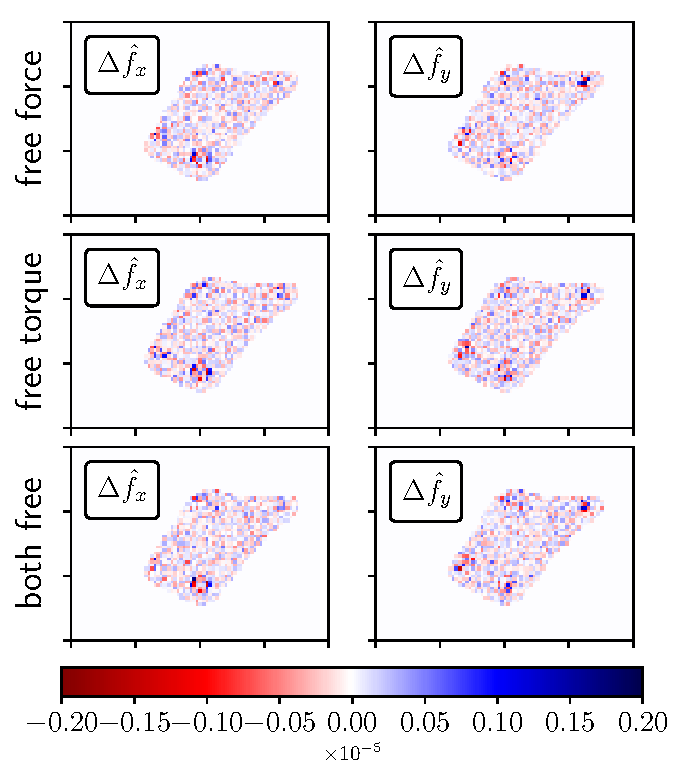
\includegraphics[width=\linewidth]{fig6}
\caption{\textbf{Constraints are unsatisfied unless enforced.} Plotted are best reconstructions
  under $\tilde{\Phi}_{L^{1}}$ penalty and the difference between
  these reconstructions and the corresponding fully constrained
  reconstruction in Fig.~\ref{COMPARE}. }
\label{fig:fig3}
\end{figure}

Finally, we explore the effects of relaxing the footprint constraint. 
By artificially expanding the footprint, we relax the 
constraint. In the 4-pad example, using the $\tilde{\Phi}_{L^{1}}$
regularizer, the footprint constraint is not 
especially critical. However, as we shall see, for stresses that are concentrated 
near the periphery of the cell footprint, 

%\begin{figure}
%%\includegraphics[width=\linewidth]{4-pad_boundary}
%\caption{\textbf{Boundary constraint weakening} leads to solutions
%  where the support does not fall naturally within the cell
%  boundary. In the unconstrained reconstruction, the support of the
%  stress was allowed to extend an additional $10$ pixels outside of
%  the cell boundary. The reconstruction did not naturally limit its
%  support to the cell boundary.}
%\label{fig:fig4}
%\end{figure}


\section{Reconstruction from single cell data}

To apply our method on high-resolution experimental data, we consider
the displacements resulting from stress generated by a single isolated
mesenchymal stem cell. The surface displacements were measured using
Hilbert space dynamometry which uses phase information of the periodic
signal arising from a chemically patterned grid on the substrate
\cite{POPESCU}.  In this dataset only $x$-displacements at a
resolution of the patterned grid spacing can be measured, as shown in
Fig.~\ref{DATA}



\begin{figure}
%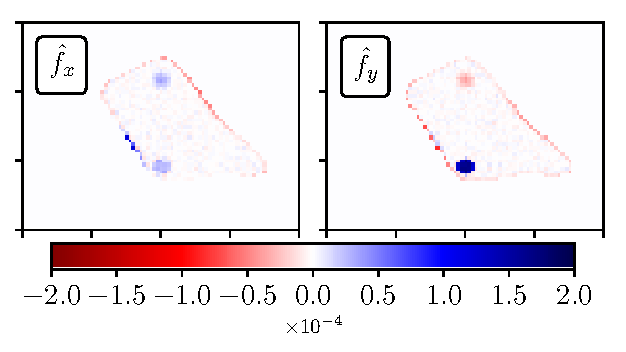
\includegraphics[width=\linewidth]{fig7}
\caption{\textbf{Footprint misspecification.} Reconstructions performed under footprint of the wrong orientation}
\label{DATA}
\end{figure}

\begin{figure}
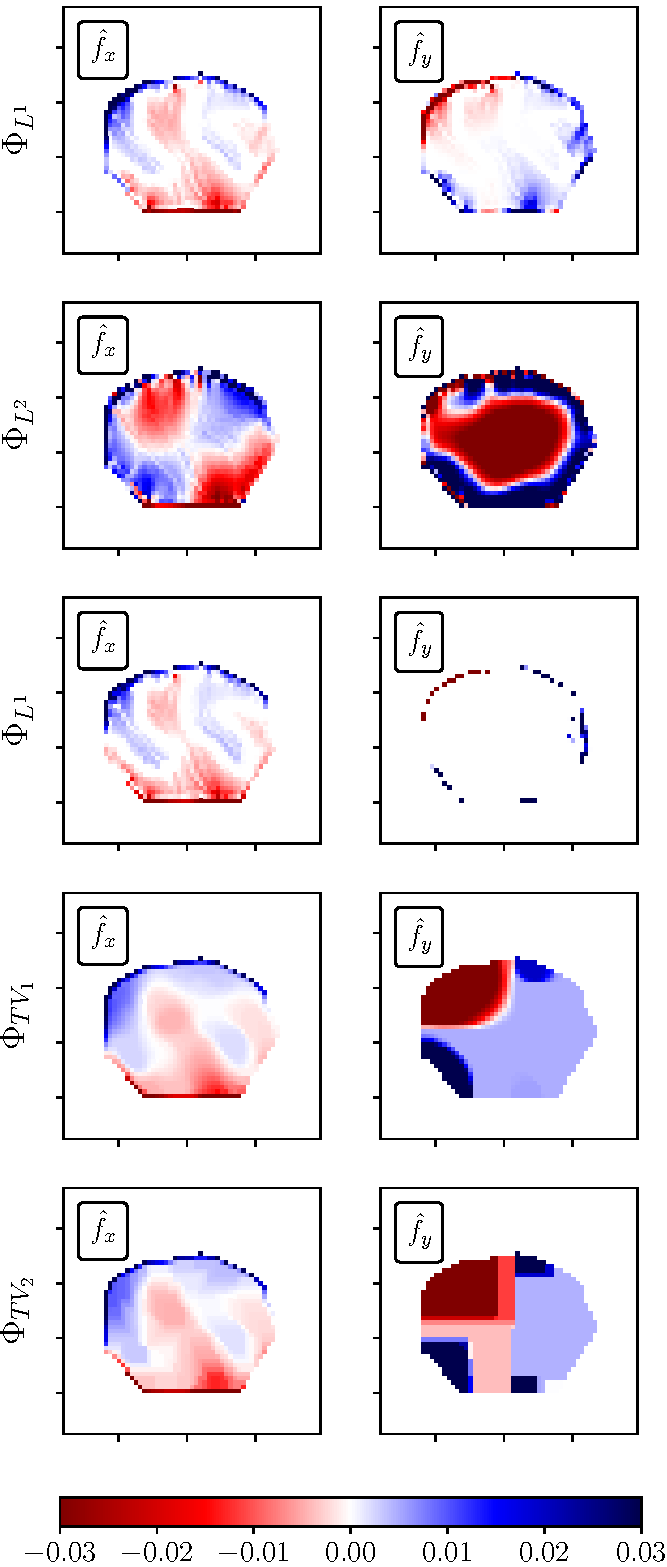
\includegraphics[width=\linewidth]{fig8}
\caption{\textbf{Mesenchymal stem cell displacement field.} Measured
 along $\hat{x}$ (the horizontal axis). Boundary of the cell (yellow) was hand-drawn
based on bright-field image of the cell.
%Raw bight
%field image of a mesenchymal stem cell. The cell footprint boundary
%is estimated from hand segmentation of the image. (b) The
%$x-$displacement fields (horizontal displacements) at the surface of the substrate. (c) The
%displacements of the patterned lines.
}
\label{DATA}
\end{figure}
%
The $\lambda-$optimal results for the reconstructed stress field
$\hat{\f}$ using the $\tilde{\Phi}_{L^{1}}$ regularization and the
full set of constraints are shown in Fig.~\ref{DATA2}.

\begin{figure}
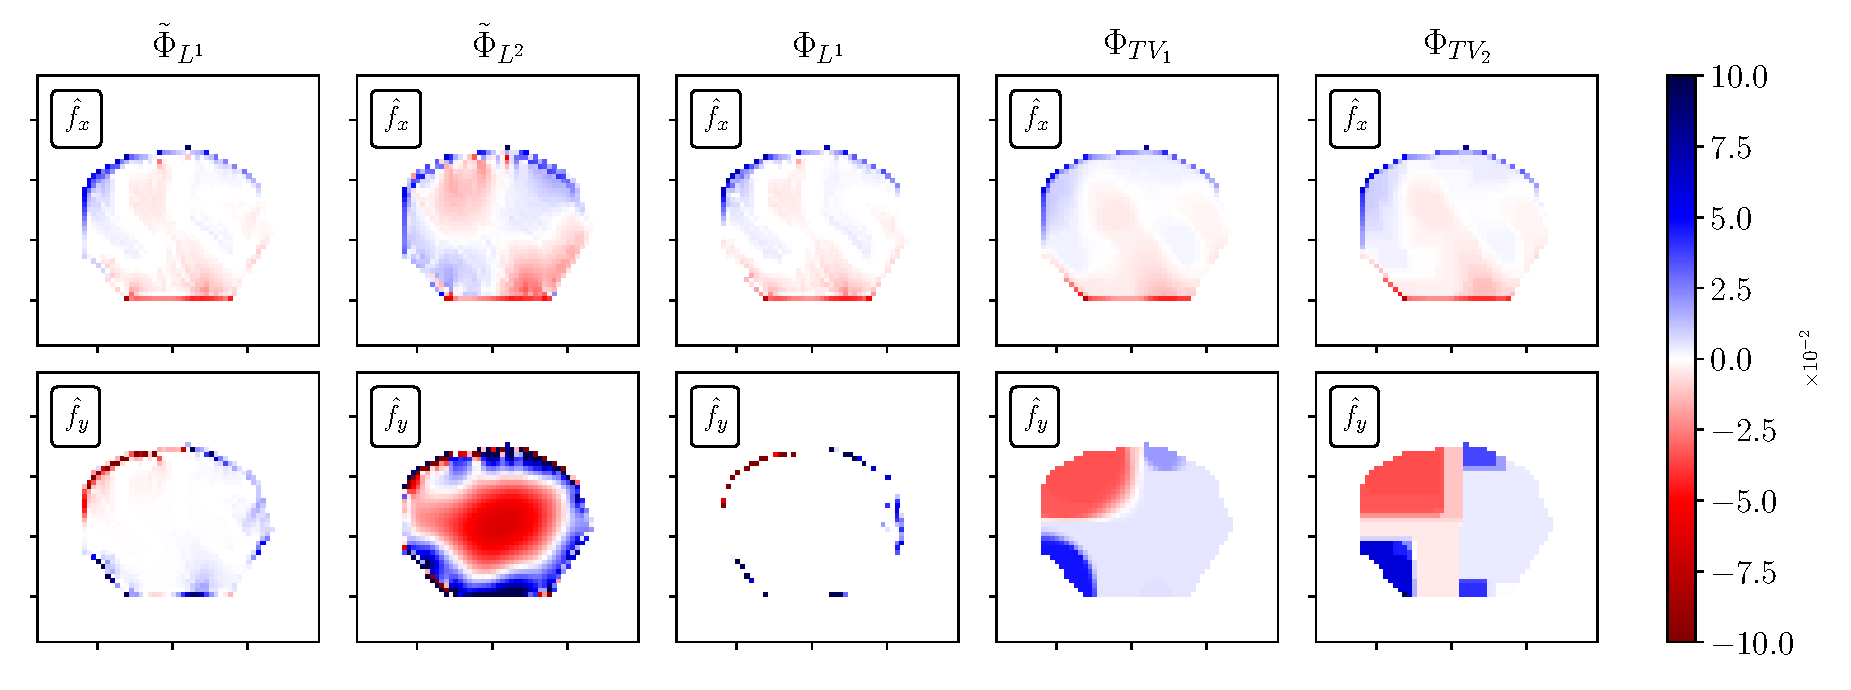
\includegraphics[width=\linewidth]{fig9}
\caption{\textbf{Reconstruction of experimental surface stress field.}
  Reconstruction of $\f$ from the measured displacements shown in
  Fig.~\ref{DATA} using the norms defined in the manuscript. In each 
  case, $\lambda$ was chosen using the L-curve method as in the appendices.}
\label{DATA2}
\end{figure}

As evident from the reconstructions, the surface forces are
concentrated near the border of the cell footprint. For such
boundary-dominated stress fields, the footprint constraint is expected
to be important in the recovery of $\f$. Fig.~\ref{DATA3} compares the
reconstruction with that computed with an artifically expanded
footprint. Using an incorrect footprint results in a force
distribution $\hat{\f}$ that differs from the ``true'' distribution,
especially near the borders.
\begin{figure}
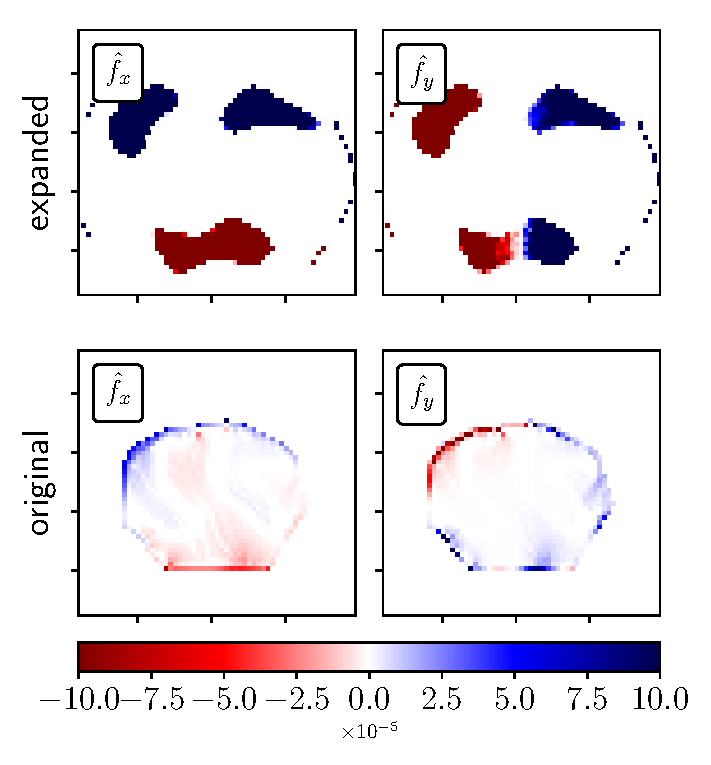
\includegraphics[width=\linewidth]{fig10}
\caption{\textbf{Modification of footprint constraint.} Comparing the
  surface force reconstruction using the estimated cell footprint
  (from the bright field image) with the reconstruction derived from a
  false cell footprint. Since the forces are concentrated near the
  cell border, the reconstruction is sensitive to the location of the
  border.}
\label{DATA3}
\end{figure}

%%%%%%%%%%%%%%%%%%%%%%%%%%%%%%%%%%%%%%%%%%%%%%%%%%%%%%%%%%%%%%%%%%
\section{Summary and Conclusions}
%%%%%%%%%%%%%%%%%%%%%%%%%%%%%%%%%%%%%%%%%%%%%%%%%%%%%%%%%%%%%%%%%%

We presented a systematic approach to solving the inverse problem
associated with the reconstruction--from displacements of the
underlying substrate--of surface stresses imparted by isolated cells.
Under piecewise affine approximations of the surface force, we
provided an exact solution to the forward problem as a system of
linear equations. This approximation to the forward problem is used in
a data mismatch term $\Phi_{\rm data}$ (Eq.~\ref{PHIDATA}).
In the numerical implementation of the optimization problem, we also
motivated the use of a cut-off in the solution of the forward problem
that greatly reduces the rank of the inverse problem thereby
decreasing both the computational complexity of the problem and the
memory requirements. This cut-off approach is appropriate only in
scenarios in which the stress-generating cell is localized and far
from the system boundaries. Assays in which cells or layers that
extend to the boundary of the sample, or in which the substrate is of
finite depth will required the careful implementation of boundary
conditions defined by the sample size.  

Upon further consideration of physical and geometric features, 
we motivated additional important terms the objective function.   
The fundamental optimization problem involves minimizing an objective
function containing $L^{1}$ regularization terms that are invariant to
coordinate rotation. The anisotropy of $\hat{\f}$ derives soley from
the anisotropy in the data. Important physical constraints including
vanishing net force/net torque and zero stress outside the cell
footprint are also imposed. By exploring the mathematical features of
the stress inference problem, we find that properly identifying and
implementing physical constraints (such as no-force and no-torque) are
key to accurate stress recovery.

We also showed how the known footprint boundary can impact the
reconstruction, especially when adhesion sites are concentrated near
the cell boundary. Such focal adhesion configurations are commonly
observed in cells grown on 2D substrates. In general, cell boundaries
that artificially extend beyond the true footprint worsens the
inversion, allowing for ``leakage'' of stress beyond its actual
support.

%In our test cases and in the analysis of an experimental dataset, we
%have assumed that the elastic properties of the substrate (Young's
%modulus and Poisson ratio) are known. These experimetal parameters can 
%also be inferred 

%%%%%%%%%%%%%%%%%%
\section{Acknowledgements}

This work was supported in part by the Intramural Research Program of the NIH.


\bibliography{refs}

\clearpage
\newpage 

\appendix
\begin{widetext}
\section{Appendix A: Elastic Green's function}

For completeness, we explicitly list the components of the Green's tensor 
for a linear elastic substrate \cite{LANDAU}

%
\begin{align}
G_{ss}(x,y,z) = \frac{1+\nu}{2\pi E}\left[\frac{2(1-\nu)R_{\perp}-z}{R_{\perp}(R_{\perp}-z)} + 
\frac{[2R_{\perp}(\nu R_{\perp}-z)+z^{2}]s^{2}}{R_{\perp}^{3}(R_{\perp}-z)^{2}}\right],
\end{align}
%\begin{equation}
%G_{yy} =\frac{1+\nu}{2\pi E}\left[\frac{2(1-\nu)R_{\perp}-z}{R_{\perp}(R_{\perp}-z)}
%+\frac{[2R_{\perp}(\nu R_{\perp}-z)+z^{2}]y^{2}}{R_{\perp}^{3}(R_{\perp}-z)^{2}}\right],
%\end{equation}
\begin{equation}
G_{zz}(x,y,z) =\frac{1+\nu}{2\pi E}\left(\frac{2(1-\nu)}
{R_{\perp}}+\frac{z^{2}}{R_{\perp}^{3}}\right),
\label{eq:Gzz0}
\end{equation}
\begin{equation} 
G_{xy}(x,y,z) = G_{yx}=\frac{1+\nu}{2\pi E}\frac{[2R_{\perp}(\nu R_{\perp}-z)+z^{2}]xy}{R_{\perp}^{3}
(R_{\perp}-z)^{2}},
\label{eq:Gxy0}
\end{equation}
\begin{equation}
G_{sz, zs}(x,y,z) =\frac{1+\nu}{2\pi E}\left(\frac{sz}{R_{\perp}^{3}}\pm\frac{(1-2\nu)s}{R_{\perp}
(R_{\perp}-z)}\right).
\end{equation}
%
where $s\equiv x,y$. The last equation with $\pm$ corresponds to
$G_{sz}$ and $G_{zs}$, respectively, and $R_{\perp} \equiv \sqrt{x^{2}
  +y^{2}}$. The Young's modulus and Poisson ratio of the elastic
substrate are denoted by $E$ and $\nu$, respectively.

\section{Appendix B: Displacements and stresses at discrete positions}

Here, we show the explicit expressions relating displacements $\u(x_{n}, y_{m})$ at 
grid points $(x_{n},y_{m})$ in terms of stress fields at the same locations. Using 
the interpolation of $\f(x,y)$ defined by Eq.~\ref{eq:sigma_affine} in 
Eq.~\ref{eq:UMODEL1s}, we find
%
\begin{align}
\lefteqn{u_x(x_n,y_m) =}  \nonumber\\
 & \quad \sum_{(x_j,y_k)\in\Omega} \Bigg\{ \Bigg[f_{x}(x_j,y_k)
- x_j\left(\frac{f_{x}(x_{j+1},y_k) - f_{x}(x_{j-1},y_k)}{2\delta x}\right)
 -y_k\left( \frac{f_{x}(x_j,y_{k+1}) -
f_{x}(x_j,y_{k-1})}{2\delta y}\right) \Bigg]{\langle G_{xx} \rangle}^{nmjk} \nonumber \\
& \qquad\qquad +\left[ \frac{f_{x}(x_{j+1},y_k) -
f_{x}(x_{j-1},y_k)}{2\delta x}\right]\langle xG_{xx} \rangle^{nmjk} 
+ \left[  \frac{f_{x}(x_j,y_{k+1}) - f_{x}(x_j,y_{k-1}) }{2\delta y} \right]
\langle yG_{xx} \rangle^{nmjk}\nonumber\\
&\qquad\qquad + \Bigg[f_{y}(x_j,y_k)-x_j\left(\frac{f_{y}(x_{j+1},y_k)-
f_{y}(x_{j-1},y_k) }{2\delta x}\right)-y_k\left( \frac{f_{y}(x_j,y_{k+1}) 
-f_{y}(x_j,y_{k-1}) }{2\delta y}\right) \Bigg] \langle G_{xy} \rangle^{nmjk}\nonumber \\
&\qquad\qquad +\left[ \frac{f_{y}(x_{j+1},y_k) - f_{y}(x_{j-1},y_k) }{2\delta x}\right]  
%\int_{y_k-\delta y/2}^{y_k+\delta y/2}\!\!
\langle xG_{xy} \rangle^{nmjk} + 
\left[\frac{f_{y}(x_j,y_{k+1}) - 
f_{y}(x_j,y_{k-1}) }{2\delta y}\right]\langle yG_{xy} \rangle^{nmjk} \Bigg\},
\label{eq:ux_decomposed}
\end{align}
%
where

\begin{align}
%\lefteqn{\langle G_{st} \rangle^{nmjk} = }\nonumber\\
%&\qquad    \int_{y_k-\delta y/2}^{y_k+\delta y/2} \int_{x_j-\delta x/2}^{x_j+\delta x/2} G_{st}(x_n-x',y_m-y') \dd x' \dd y' \label{eq:G_ave} \\
\langle g(x,y)G_{uv} \rangle^{nmjk} = \int_{y_k-\delta y/2}^{y_k+\delta y/2} 
\int_{x_j-\delta x/2}^{x_j+\delta x/2} g(x',y')
G_{uv}(x_n-x',y_m-y')\dd x'\dd y', \label{eq:G_ave} 
\end{align}
%
except that at the edges where we use one-sided differences so that we
are only differentiating within $\Omega$. A similar expression can be
found for solving for $u_y$ (not shown). Collecting terms, we 
write $u_{x,y}(x_{n},y_{m})$ in terms of $\f(x_{j}, y_{k})$ 
in Eq.~\ref{eq:linearsystem1}, where 

\begin{align}
X^{nmjk} & = \langle G_{xx} \rangle^{nmjk} - 
\langle G_{xx}\rangle^{n,m,j-1,k}\frac{x_{j-1}}{2\delta x}
+ \langle G_{xx} \rangle^{n,m,j+1,k}\frac{x_{j+1}}{2\delta x} 
-  \langle G_{xx} \rangle^{n,m,j,k-1}\frac{y_{k-1}}{2\delta y}  \nonumber\\
\: &\quad + \langle G_{xx} \rangle^{n,m,j,k+1}\frac{y_{k+1}}{2\delta y} 
-\frac{\langle xG_{xx} \rangle^{n,m,j-1,k}}{2\delta x}
+\frac{\langle xG_{xx} \rangle^{n,m,j+1,k}}{2\delta x} 
- \frac{\langle yG_{xx} \rangle^{n,m,j,k-1}}{2\delta y} 
+\frac{\langle yG_{xx} \rangle^{n,m,j,k+1}}{2\delta y}, 
\label{eq:linearsystemX}
\end{align}
\begin{align}
Y^{nmjk} & =  \langle G_{xy} \rangle^{nmjk} 
- \langle G_{xy} \rangle^{n,m,j-1,k}\frac{x_{j-1}}{2\delta x}
+\langle G_{xy} \rangle^{n,m,j+1,k}\frac{x_{j+1}}{2\delta x} 
- \langle G_{xy} \rangle^{n,m,j,k-1}\frac{y_{k-1}}{2\delta y} \nonumber\\
\: & \quad+\langle G_{xy} \rangle^{n,m,j,k+1}\frac{y_{k+1}}{2\delta y}  
-\frac{\langle xG_{xy} \rangle^{n,m,j-1,k}}{2\delta x}+
\frac{\langle xG_{xy} \rangle^{n,m,j+1,k}}{2\delta x} 
- \frac{\langle yG_{xy} \rangle^{n,m,j,k-1}}{2\delta y} 
+\frac{\langle yG_{xy} \rangle^{n,m,j,k+1}}{2\delta y}.
\label{eq:linearsystemY}
\end{align}
%
Explicit closed-form expressions for the integrals in
Eq.~\ref{eq:G_ave} are given below. By defining $\Delta x_{nj}^+ = x_n -
(x_j+\delta x/2),$ $\Delta x_{nj}^- = x_n - (x_j-\delta x/2)$, $\Delta
y_{mk}^+ = y_m - (y_k+\delta y/2)$, and $\Delta y_{mk}^+ = y_m -
(y_k-\delta y/2)$, we find

\begin{align}
\langle G_{uv}\rangle^{nmjk} &=   g_{uv}( \Delta x_{nj}^+,\Delta y_{mk}^+) - g_{uv}( \Delta x_{nj}^+,\Delta y_{mk}^-)
-g_{uv}(\Delta x_{nj}^-, \Delta y_{mk}^+) + g_{uv}(\Delta x_{nj}^- , \Delta y_{mk}^-)
\end{align}
where
\begin{align}
g_{xx}(x,y) &= \frac{\nu+1}{\pi E}\Bigg[ x(1-\nu ) \log\left( \sqrt{x^2+y^2}+y\right)
+ y \log\left(\sqrt{x^2+y^2} +x\right)-y  \Bigg] \label{eq:fxx} \\
g_{yy}(x,y) &= \frac{\nu+1}{\pi E}\Bigg[ y(1-\nu ) \log\left( \sqrt{x^2+y^2}+x\right)
+ x \log\left(\sqrt{x^2+y^2} +y\right)-x  \Bigg] \label{eq:fyy} \\
g_{xy}(x,y) &= -\frac{\nu(\nu+1)}{\pi E}\sqrt{x^2+y^2}. \label{eq:fxy}
\end{align}
%
The first moments are

\begin{align}
\langle xG_{xx}(x,y) \rangle^{nmjk} & =\Big[g_{xx}(\Delta x_{nj}^+,\Delta y_{mk}^+)
- g_{xx}(\Delta x_{nj}^+,\Delta y_{mk}^-)
-g_{xx}(\Delta x_{nj}^-, \Delta y_{mk}^+)+ g_{xx}
(\Delta x_{nj}^- , \Delta y_{mk}^-)\Big] x_n\nonumber\\
\: &\qquad - \Big[g^x_{xx}( \Delta x_{nj}^+ , \Delta y_{mk}^+)- 
g^x_{xx}(\Delta x_{nj}^+ , \Delta y_{mk}^-)-
g^x_{xx}(\Delta x_{nj}^-, \Delta y_{mk}^+) + 
g^x_{xx}(\Delta x_{nj}^- , \Delta y_{mk}^-)\Big],
\end{align}
%
where

\begin{align}
g^x_{xx}(x,y) &= \frac{\nu+1}{2\pi E} \Big[ (\nu+1)y\sqrt{x^2 + y^2}
- (\nu-1) x^2\log\left(\sqrt{x^2 + y^2} +y  \right)  \Big],\label{eq:fxxx}
\end{align}

\begin{align}
\langle yG_{xx}(x,y) \rangle^{nmjk} & = 
\Big[g_{xx}(\Delta x_{nj}^{+},\Delta y_{mk}^+)-g_{xx}(\Delta x_{nj}^+,\Delta y_{mk}^-)
-g_{xx}(\Delta x_{nj}^{-}, \Delta y_{mk}^+) + 
g_{xx}(\Delta x_{nj}^{-}, \Delta y_{mk}^-)\Big] y_m\nonumber\\
\: &\qquad - \Big[ g^y_{xx}(\Delta x_{nj}^+,\Delta y_{mk}^+) 
- g^y_{xx}(\Delta x_{nj}^+,\Delta y_{mk}^-)
- g^y_{xx}(\Delta x_{nj}^-,\Delta y_{mk}^+) 
+ g^y_{xx}(\Delta x_{nj}^-,\Delta y_{mk}^-)\Big],
\end{align}
%
where

\begin{align}
g^y_{xx}(x,y) &=\frac{\nu+1}{2\pi E} \Bigg[y^2\log\left(\sqrt{x^2+y^2}+x \right)
-\sqrt{x^2+y^2}\left((2\nu-1)x + \frac{1}{2}\sqrt{x^2+y^2} \right)  \Bigg], \label{eq:fyxx}
\end{align}
%
and

\begin{align}
\langle xG_{xy}(x,y)\rangle^{nmjk} & = 
\Big[g_{xy}(\Delta x_{nj}^{-},\Delta y_{mk}^+)-g_{xy}(\Delta x_{nj}^{-},\Delta y_{mk}^-)
- g_{xy}(\Delta x_{nj}^{+},\Delta y_{mk}^+) + g_{xy}(\Delta x_{nj}^+,\Delta y_{mk}^-) \Big]x_n \nonumber\\
\: & \qquad -\Big[g_{xy}^x(\Delta x_{nj}^{+},\Delta y_{mk}^+) - g_{xy}^x(\Delta x_{nj}^{+},\Delta y_{mk}^-)
-g_{xy}^x(\Delta x_{nj}^{-},\Delta y_{mk}^+)+g_{xy}^x(\Delta x_{nj}^{-},\Delta y_{mk}^-)\Big]
\end{align}
%
where

\begin{align}
g_{xy}^x(x,y) &=\frac{\nu(\nu+1)}{\pi E}\Big[ \frac{y^2}{2}\log\left(\sqrt{x^2+y^2} +x\right)
-\frac{1}{4}\sqrt{x^2+y^2}\left(\sqrt{x^2+y^2}+2x\right) \Big]. \label{eq:fxxy}
\end{align}
All of these expressions may be found through direct iterated
evaluation of the integrals, noting that as long as $n\neq m$ or
$j\neq k$ the integrand (effectively the Green's function) is bounded,
hence making Fubini's theorem applicable given the compactly supported
domains of integration.

In the special case where $n=m$ and $j=k$, these formulae also
hold. This fact is found by decomposing the integration domain to
exclude the origin, for instance in the manner
\begin{equation}
\int_{ -\Delta y/2 }^{\Delta y/2 }\int_{- \Delta x/2 }^{\Delta x/2 } \d\r = 
\lim_{\varepsilon\to0} \left( \int_\varepsilon^{\Delta y/2}  
+  \int_{-\Delta y/2}^\varepsilon   \right)\int_{\Delta x/2}^{\Delta x/2} \d\r.~\label{eq:splitdomain}
\end{equation}
Since the antiderivatives of
Eqs~\ref{eq:fxx},~\ref{eq:fyy},~\ref{eq:fxy},~\ref{eq:fxxx},~\ref{eq:fyxx},
and~\ref{eq:fxxy} all have well-defined limits with only removable
discontinuities at the origin, integrals of the Green's functions
defined through Eq.~\ref{eq:splitdomain} all converge about the origin
and the equations above also hold in the case where $n=m$ and $j=k$.
These explicit expressions allow us to accurately evaluate
$\u(\r_{i})$ in $\Phi_{\rm data}[\f]$.

\section{Appendix C: Decay of displacement fields}

Note that $u_x$ and $u_y$ are symmetric in form. Hence, it will
suffice to prove just one of these assertions. Eq.~\ref{eq:UMODEL1s}
can be written as

\begin{align}
u_x(\r) & = \frac{1+\nu}{\pi E} \int \frac{\dd \r}{|\r-\r'|} 
\Bigg\{ \left[ \frac{\nu(x - x')^2}{|\r-\r'|^2} + 1-\nu \right]f_{x}(\r') +
\nu\frac{(x-x')(y-y')}{|\r-\r'|^2} f_y(\r')  \Bigg\} \nonumber\\
& \equiv \frac{1+\nu}{\pi E}   \int\frac{\rho_x(\r,\r')}{|\r-\r'|} \dd \r'  \label{eq:rhoeq}
\end{align}
where $\rho_x(\r,\r')$ is $\mathcal{O}(1)$ as
$\vert\r\vert\to\infty$. Without loss of generality, we assume that
the coordinate system is centered at some point
$\mathbf{0}\in\Omega$. The Euclidean distances can then be represented
through the binomial expansion,

\begin{align}
\frac{1}{|\r-\r'|^p} &= \frac{1}{|\r|^p}\frac{1}{\left(1 - \frac{2\r\cdot\r'}{|\r|^2} 
+\frac{\vert\r'\vert^{2}}{\vert\r\vert^{2}}\right)^{p/2}} = \frac{1}{|\r|^p}\sum_{k=0}^\infty {{{p\over 2}+k-1}\choose{k}} 
{\left( \underbrace{ \frac{2\r\cdot\r' - |\r'|^2}{|\r|^2}}_{\mathcal{O}(|\r|^{-1})} \right)}^k.
\end{align}
% 
Since $\r\not\in\Omega$ and $\r'\in\Omega$, the series converges in
the $\vert \r\vert \to \infty$ limit. Plugging this series into the
last line of Eq.~\ref{eq:rhoeq}, where $p=1$, one sees that it in order to show
that the magnitude of $u_x(\r)$ is $\mathcal{O}(|\r|^{-q})$, it
suffices to show that $\int \rho(\r,\r')\dd\r' \leq
{\cal O}(|\r|^{-q+1})$.

Using the fact that $\int \f(\r)\d\r = \mathbf{0}$, one finds that
%
\begin{align}
\int \rho_{x}(\r,\r')\d\r'  & =  \int (1-\nu)f_x(\r')\d\r'
+\nu\int\left[\frac{(x - x')^2}{|\r-\r'|^2} f_{x}(\r') +
\frac{(x-x')(y-y')}{|\r-\r'|^2} f_y(\r')  \right]\d\r' \nonumber\\
\: &= \frac{\nu}{|\r|^2}\int\Bigg[(x - x')^2f_{x}(\r')
+ (x-x')(y-y')f_y(\r')  \Bigg]
\sum_{k=0}^\infty \left[\frac{2\r\cdot\r' - |\r'|^2}{|\r|^2} \right]^k \d\r'.
\end{align}
%
Expanding the leading order term of this expression, we see that

\begin{align*}
\int\rho_{x}(\r,\r')\d\r 
&= \frac{\nu}{|\r|^2}\int\Bigg[(x- x')^2f_{x}(\r')+(x-x')(y-y')f_y(\r')\Bigg]
\d\r' \nonumber\\
\: &= \frac{\nu}{|\r|^2}  \Bigg[  -2x\int x' f_x(\r')\d\r'  + \int x'^2 f_x(\r')\d\r'- x\int y' f_y(\r') \d\r'
- y\int x' f_y(\r')\d\r'
+ \int x'y' f_y(\r') \d\r'\Bigg] \nonumber \\
\: & =\mathcal{O}(|\r|^{-1}).
\end{align*}
%
Hence, it is evident that this integral of $\mathcal{O}(|\r|^{-2})$,
where to the leading order we have

\begin{align}
\lefteqn{u_x(\r) = \frac{1+\nu}{\pi E |\r|^2}
\Bigg[ -2\nu\frac{x}{|\r|}\int x' f_x(\r')\d\r'
-\frac{x\nu}{|\r|}\int y' f_y(\r') \d\r'  }\nonumber\\
&\qquad- \frac{y\nu}{|\r|}\int x' f_y(\r')\d\r' 
+ (1-\nu)\frac{\r}{|\r|}\cdot\int \r' f_x(\r') \d\r'\Bigg] + \mathcal{O}(|\r|^{-3})
\end{align}


% and $\cos\theta = \frac{(\r-\r_0,\r'-\r_0)} {|\r - \r_0| |\r'-\r_0|}$. Eq.~\ref{eq:multipole}  is obtained through binomial expansion of the Euclidean distance functions in the denominators of Eq.~\ref{eq:Gzz0} and Eq.~\ref{eq:Gxy0},
%\begin{align*}
%\lefteqn{|\r - \r'|^s = |\r-\r_0 - (\r'-\r_0) |^s }\\
%&\quad= \left[ |\r-\r_0|^2 -2 (\r-\r_0)(\r'-\r_0) + |\r'-\r_0|^2  \right]^{s/2}.
%\end{align*}
%In particular, since all the Green's functions scale with distance as $|\r-\r'|^{-1}$, we have the following approximation through the binomial expansion
%\begin{align}
%\lefteqn{\frac{1}{|\r-\r'|} =} \nonumber\\
%&  \frac{1}{|\r-\r_0|}\sum_{n=0}^\infty {n-\frac{1}{2} \choose n} \left[  \frac{2 (\r-\r_0)(\r'-\r_0) - |\r'-\r_0|^2 }{|\r-\r_0|} \right]^n \nonumber\\
%&=\frac{1}{|\r-\r_0|}\Bigg\{ 1 +    \frac{2 (\r-\r_0)(\r'-\r_0) - |\r'-\r_0|^2 }{2|\r-\r_0|}    \nonumber\\
%&\qquad+ \mathcal{O}(|\r-\r_0|^{-2})\Bigg\}.
%\end{align}
%Invoking the net force-free constraint, the first few terms of the expansion of Eq.~\ref{eq:multipole} are
%\begin{align}
%U_0 = 0
%\end{align}

      
%\subsection{Proof of~Lemma \ref{lem:affine_error}}
%
%Let $\tilde{\bsigma}$ be the piecewise affine approximation of the stress field $\bsigma$, and $\r\in\Omega_{jk}$. Then,
%by the Taylor remainder theorem, one sees that
%$$
%\sigma_{x}(\r) - \tilde{\sigma}_x(\r) = \frac{1}{2}(\r-\r_{jk})^\intercal\d^2\sigma_{x}(\mathbf{c}_{jk})(\r-\r_{jk})
%$$
%and
%$$
%\sigma_{y}(\r) - \tilde{\sigma}_x(\r) = \frac{1}{2}(\r-\r_{jk})^\intercal\d^2\sigma_{x}(\mathbf{a}_{jk})(\r-\r_{jk})
%$$
%where $\mathbf{c}_{jk},\mathbf{a}_{jk}\in\Omega_{jk}$ and $\r_{jk}\in\Omega_{jk}$ is the point about which interpolation is performed.
%Hence,
%{\small
%\begin{align}
%\lefteqn{u_x(\r) - \tilde{u}_x(\r)  = \sum_{j,k}\int_{\Omega_{jk}} G_{xx} (\r,\r')(\sigma_{x}(\r') - \tilde{\sigma}_x(\r')) \d\r 
% +\sum_{j,k}\int_{\Omega_{jk}} G_{xy} (\r,\r')(\sigma_{y}(\r') - \tilde{\sigma}_y(\r')) \d\r } \nonumber\\
%&= \sum_{j,k} \frac{\d_{xx}^2\sigma_x(\mathbf{c}_{jk})}{2}\int_{\Omega_{jk}} G_{xx}(x-x',y-y')  (x'-x_j)^2 \d\r + \sum_{j,k} {\d_{xy}^2\sigma_x(\mathbf{c}_{jk})}\int_{\Omega_{jk}} G_{xx}(x-x',y-y')  (x'-x_j)(y'-y_k)\d\r \nonumber\\
%&\quad + \sum_{j,k} \frac{\d_{yy}^2\sigma_x(\mathbf{c}_{jk})}{2}\int_{\Omega_{jk}} G_{xx}(x-x',y-y')  (y'-y_k)^2\d\r   + \sum_{j,k} \frac{\d_{xx}^2\sigma_y(\mathbf{a}_{jk})}{2}\int_{\Omega_{jk}} G_{xy}(x-x',y-y')  (x'-x_j)^2\d\r \nonumber\\
%&  + \sum_{j,k} {\d_{xy}^2\sigma_y(\mathbf{a}_{jk})}\int_{\Omega_{jk}} G_{xy}(x-x',y-y')  (x'-x_j)(y'-y_k)\d\r + \sum_{j,k} \frac{\d_{yy}^2\sigma_y(\mathbf{a}_{jk})}{2}\int_{\Omega_{jk}} G_{xy}(x-x',y-y')  (y'-y_k)^2\d\r 
%\end{align}
%}
%
%\subsection{Proof of~Theorem \ref{thm:main}}
%
%Consider the data penalty term $\Phi_{\textrm{data}}$ of the optimization problem
%\begin{align*}
%\Phi_{\rm data}[\bs] &=\sum_{i=1}^{M}\vert \u^{\rm
%  data}(\r_{i})- \u(\r_i)\vert^{2}  + \sum_{i=M+1}^{N}\vert \u^{\rm
%  data}(\r_{i})- \u(\r_i)\vert^{2} 
%\end{align*}
%where the first $M$ data points are all within a maximal cut off distance of $R$ within the boundary of the cell and the remaining $N-M$ datapoints lie outside this distance.
%
%

\end{widetext}
%%%%%%%%%%%%%%%%%%%%%%%%%%%%%%%%%%%%%%%%%%%%%%%%%%%%%%%%%%%%%%%%%%%%%%%%
%%%%%%%%%%%%%%%%%%%%%%%%%%%%%%%%%%%%%%%%%%%%%%%%%%%%%%%%%%%%%%%%%%%%%%%%
\end{document}
%%%%%%%%%%%%%%%%%%%%%%%%%%%%%%%%%%%%%%%%%%%%%%%%%%%%%%%%%%%%%%%%%%%%%%%%
%%%%%%%%%%%%%%%%%%%%%%%%%%%%%%%%%%%%%%%%%%%%%%%%%%%%%%%%%%%%%%%%%%%%%%%%

